%%
%% This is file `sample-acmtog.tex',
%% generated with the docstrip utility.
%%
%% The original source files were:
%%
%% samples.dtx  (with options: `acmtog')
%% 
%% IMPORTANT NOTICE:
%% 
%% For the copyright see the source file.
%% 
%% Any modified versions of this file must be renamed
%% with new filenames distinct from sample-acmtog.tex.
%% 
%% For distribution of the original source see the terms
%% for copying and modification in the file samples.dtx.
%% 
%% This generated file may be distributed as long as the
%% original source files, as listed above, are part of the
%% same distribution. (The sources need not necessarily be
%% in the same archive or directory.)
%%
%%
%% Commands for TeXCount
%TC:macro \cite [option:text,text]
%TC:macro \citep [option:text,text]
%TC:macro \citet [option:text,text]
%TC:envir table 0 1
%TC:envir table* 0 1
%TC:envir tabular [ignore] word
%TC:envir displaymath 0 word
%TC:envir math 0 word
%TC:envir comment 0 0
%%
%%
%% The first command in your LaTeX source must be the \documentclass command.
\documentclass[acmtog]{acmart}
\usepackage{subcaption}

%%
%% \BibTeX command to typeset BibTeX logo in the docs
\AtBeginDocument{%
  \providecommand\BibTeX{{%
    \normalfont B\kern-0.5em{\scshape i\kern-0.25em b}\kern-0.8em\TeX}}}

%% Rights management information.  This information is sent to you
%% when you complete the rights form.  These commands have SAMPLE
%% values in them; it is your responsibility as an author to replace
%% the commands and values with those provided to you when you
%% complete the rights form.
\setcopyright{acmcopyright}
\copyrightyear{2018}
\acmYear{2018}
\acmDOI{XXXXXXX.XXXXXXX}


%%
%% These commands are for a JOURNAL article.
\acmJournal{TOG}
\acmVolume{37}
\acmNumber{4}
\acmArticle{111}
\acmMonth{8}

%%
%% Submission ID.
%% Use this when submitting an article to a sponsored event. You'll
%% receive a unique submission ID from the organizers
%% of the event, and this ID should be used as the parameter to this command.
%%\acmSubmissionID{123-A56-BU3}

%%
%% The majority of ACM publications use numbered citations and
%% references.  The command \citestyle{authoryear} switches to the
%% "author year" style.
%%
%% If you are preparing content for an event
%% sponsored by ACM SIGGRAPH, you must use the "author year" style of
%% citations and references.
\citestyle{acmauthoryear}

%%
%% end of the preamble, start of the body of the document source.
\begin{document}

%%
%% The "title" command has an optional parameter,
%% allowing the author to define a "short title" to be used in page headers.
\title{Encouraging emotion regulation in social media conversations through self-reflection}

%%
%% The "author" command and its associated commands are used to define
%% the authors and their affiliations.
%% Of note is the shared affiliation of the first two authors, and the
%% "authornote" and "authornotemark" commands
%% used to denote shared contribution to the research.
\author{Ben Trovato}
\authornote{Both authors contributed equally to this research.}
\email{trovato@corporation.com}
\orcid{1234-5678-9012}
\author{G.K.M. Tobin}
\authornotemark[1]
\email{webmaster@marysville-ohio.com}
\affiliation{%
  \institution{Institute for Clarity in Documentation}
  \streetaddress{P.O. Box 1212}
  \city{Dublin}
  \state{Ohio}
  \country{USA}
  \postcode{43017-6221}
}

\author{Lars Th{\o}rv{\"a}ld}
\affiliation{%
  \institution{The Th{\o}rv{\"a}ld Group}
  \streetaddress{1 Th{\o}rv{\"a}ld Circle}
  \city{Hekla}
  \country{Iceland}}
\email{larst@affiliation.org}

\author{Valerie B\'eranger}
\affiliation{%
  \institution{Inria Paris-Rocquencourt}
  \city{Rocquencourt}
  \country{France}
}



% \author{Huifen Chan}
% \affiliation{%
%   \institution{Tsinghua University}
%   \streetaddress{30 Shuangqing Rd}
%   \city{Haidian Qu}
%   \state{Beijing Shi}
%   \country{China}}

% \author{Charles Palmer}
% \affiliation{%
%   \institution{Palmer Research Laboratories}
%   \streetaddress{8600 Datapoint Drive}
%   \city{San Antonio}
%   \state{Texas}
%   \country{USA}
%   \postcode{78229}}
% \email{cpalmer@prl.com}

% \author{John Smith}
% \affiliation{%
%   \institution{The Th{\o}rv{\"a}ld Group}
%   \streetaddress{1 Th{\o}rv{\"a}ld Circle}
%   \city{Hekla}
%   \country{Iceland}}
% \email{jsmith@affiliation.org}

% \author{Julius P. Kumquat}
% \affiliation{%
%   \institution{The Kumquat Consortium}
%   \city{New York}
%   \country{USA}}
% \email{jpkumquat@consortium.net}

%%
%% By default, the full list of authors will be used in the page
%% headers. Often, this list is too long, and will overlap
%% other information printed in the page headers. This command allows
%% the author to define a more concise list
%% of authors' names for this purpose.
\renewcommand{\shortauthors}{Trovato and Tobin, et al.}

%%
%% The abstract is a short summary of the work to be presented in the
%% article.
\begin{abstract}
%   A clear and well-documented \LaTeX\ document is presented as an
%   article formatted for publication by ACM in a conference proceedings
%   or journal publication. Based on the ``acmart'' document class, this
%   article presents and explains many of the common variations, as well
%   as many of the formatting elements an author may use in the
%   preparation of the documentation of their work.
\end{abstract}

%%
%% The code below is generated by the tool at http://dl.acm.org/ccs.cfm.
%% Please copy and paste the code instead of the example below.
%%
\begin{CCSXML}
<ccs2012>
 <concept>
  <concept_id>10010520.10010553.10010562</concept_id>
  <concept_desc>Computer systems organization~Embedded systems</concept_desc>
  <concept_significance>500</concept_significance>
 </concept>
 <concept>
  <concept_id>10010520.10010575.10010755</concept_id>
  <concept_desc>Computer systems organization~Redundancy</concept_desc>
  <concept_significance>300</concept_significance>
 </concept>
 <concept>
  <concept_id>10010520.10010553.10010554</concept_id>
  <concept_desc>Computer systems organization~Robotics</concept_desc>
  <concept_significance>100</concept_significance>
 </concept>
 <concept>
  <concept_id>10003033.10003083.10003095</concept_id>
  <concept_desc>Networks~Network reliability</concept_desc>
  <concept_significance>100</concept_significance>
 </concept>
</ccs2012>
\end{CCSXML}

\ccsdesc[500]{Computer systems organization~Embedded systems}
\ccsdesc[300]{Computer systems organization~Redundancy}
\ccsdesc{Computer systems organization~Robotics}
\ccsdesc[100]{Networks~Network reliability}

%%
%% Keywords. The author(s) should pick words that accurately describe
%% the work being presented. Separate the keywords with commas.
\keywords{datasets, neural networks, gaze detection, text tagging}


%%
%% This command processes the author and affiliation and title
%% information and builds the first part of the formatted document.

%%%%%%%%%%%%%%%%%%%%%%%%%%%%%%%%%%%%%%%%%%%%%%%%%%%%%%%%%%%%%%%%%%%%%%%%%%%%%%%%%%%%%%%%%%%%%%%%%%%%%



\maketitle

\section{Introduction}
The practice of consciously modifying one's affective state is called emotion regulation. The ability to successfully perform emotion regulation is essential to function effectively in everyday life, to act appropriately in everyday interactions, or merely for hedonic purposes \cite{wadley2020digital}. The topic has been thoroughly explored in the field of psychological work, the study of cognitive behaviour as well as mental health \cite{mcrae2020emotion}, \cite{gross2015emotion}, \cite{gross2014emotion}. Owing to the boost in technology and access to digital media which provides a wide range of options available at ease, this practice of regulating emotions through the use of digital media has seen tremendous growth recently. 


Digital technologies provide a greater range of strategic options that can be easily and effectively executed. Individuals combine a variety of applications and devices for purposefully managing emotions in daily life \cite{smith2022digital}. Some examples include listening to uplifting music while exercising, watching comedy or light-hearted videos to relieve stress after work, playing social video games when feeling lonely or scrolling through social media applications to combat boredom. Social media applications are widely used by people, multiple times throughout the day. These applications contain several emotional affordances (expressible, shareable, consumable, and assessable), all of which can influence emotions as well as a behaviour associated with emotions \cite{steinert2022emotions}. Owing to its vast usage, activities on social media applications significantly impact online well-being. The prevalence of toxicity and hate speech in online conversations has been largely observed and studied in recent years. Social media conversations are fuelled by connective action and fast information spread and have given rise to online movements and debates, the results of which have affected offline events \cite{saveski2021structure}, \cite{mirbabaie2021development}. Recently, people have started being vocal about how the hate received online impacts their daily lives and questions their safety online. Posts from political people in power, news websites and young content creators, to name a few, are victims of this. It has been discovered that encountering or dealing with disrespectful or rude behaviour online is now considered standard and a part of the deal \cite{thomas2022s}. There have been some rules enforced by social media applications where accounts with a large number of followers and engagement were banned to curb the spread of offensive speech, but toxicity is still prevailing as it arises from the actions of many mildly toxic people as opposed to a few highly toxic ones \cite{saveski2021structure}. 



It is essential to ensure that social media platforms offer a safe space for healthy interaction and communication by managing the vulnerabilities to digital wellbeing. Previous studies in the field of social media and emotion regulation have focused on how social media facilitates online emotions and their effects on eudaimonic well-being \cite{goldenberg2020digital}, \cite{steinert2021corona}, \cite{yang2020social}, \cite{yue2022passive}. These include investigating how maladaptive emotion regulation methods affect problematic use of social media and smartphones, as well as determining how informed smartphone use can improve effective emotion regulation and social competence \cite{zsido2021role}. Prior research has also found that both active and passive social media usage have the potential to be procrastination or recovery activities depending on the automaticity and situational social media aspects \cite{hossain2022motivational}. \cite{ments2021second} present a second-order adaptive brain network model to simulate the process of emotion regulation in social media and discover how, while some emotion regulation strategies are protective in the short term, using them consistently results in worsened mood and relatively low well-being. Studies have also examined the user interfaces of social media applications and recommended design frameworks to assist emotion regulation in breaking the habit of making unpleasant comments on social media platforms by automatically identifying emotional aspects, such as the audience's anticipated emotional response to users' comments \cite{kiskola2021applying}.



Although these developments provide significant insights into how the process of emotion regulation unfolds in social media applications, there is a lack of digital solutions available for implementation. Current tools for emotion regulation include mood-based recommendation systems and reminders, which can only provide temporary assistance and are difficult to incorporate into daily life \cite{wadley2020digital}, \cite{slovak2022designing}. Additionally, there is a lack of a common prototype for synthesising emotion regulation because the majority of recent research in the field of digital emotion regulation is based on field studies, ecological momentary assessments (EMA), or physiological sensors combined with facial data, making it difficult to extend and replicate for further research \cite{ruensuk2020you}. It is also necessary to understand how to identify the need for emotion regulation in online environments. This entails the creation of a solution that informs users of their micro-impacts on a post, rather than providing a broad overview of "what may be the consequence." This information about one's impact will call their anonymity on a post into question and encourage them to act responsibly.


This work presents an innovative approach to delivering information regarding the need to regulate one's emotions and guiding them through the emotion regulation experience, in social media conversations, intending to embed the learning into their lives through repetitive application and, as a result, enhance online well-being. Because this study was conducted using publicly available data, it provides a foundation for expansion, extension, comparison, and contrast. Therefore, the main contributions of this work are:
\begin{itemize}
    \item We introduce a model for on-the-spot attention and response modulation support in online conversations by encouraging self-reflection in moments of ongoing highly elevated emotional expression.
    \item We propose a graph-based framework for identifying the need for emotion regulation in online social media conversations.
    \item We present design implications for social media applications to incorporate support for users' emotion regulation.
\end{itemize}
The remainder of this paper is structured as follows. We begin by reviewing recent developments in the literature, followed by a detailed description of the terms and methodologies used in this study, and finally, we summarise our research design. Then we present the results of the experiment and analysis before summarising the conclusion.


%%%%%%%%%%%%%%%%%%%%%%%%%%%%%%%%%%%%%%%%%%%%%%%%%%%%%%%%%%%%%%%%%%%%%%%%%%%%%%%%%%%%%%%%%%%%%%%%%%%%%
\section{Related work}

\subsection{Digital Emotion Regulation}
Recent DER research can be divided into three categories. The first category contains observational studies that examine how people use social media apps such as video streaming platforms, discussion forums, online games, and music to regulate their emotions, thoughts, and behaviours. Several diary studies have been undertaken to better understand various elements of everyday emotion regulation in isolation, such as the usage of social media to overcome homesickness and university students' use of music streaming platforms. Individuals' multitasking and passive scrolling habits on social media apps have also been investigated in studies revealing how people voluntarily take breaks from social media to mitigate negativity or maintain a sense of equilibrium, as well as highlighting the practice of interpersonal emotion regulation in discussion forums. The majority of studies on how digital media is used to regulate emotions have relied on self-reported questionnaires or a diary-keeping technique. Participants in this kind of data collection are required to document their interactions with emotion regulation and technology use over a given period, and then discuss their use of technology and the emotional reactions that accompany it in an interview. By limiting the amount of data that may be recorded, this strategy allows participants to track and reflect on significant insights into both work and social life. Overall, these studies reveal that people use a variety of digital technologies for emotion regulation in everyday life, emphasising the importance of the technology packed inside these devices and the need to promote well-being online.

The second category includes the design and development of new tools for DER. This field of research focuses on the creation of interventions that aim to support, improve, or guide emotion regulation skills, or to assist individuals in applying such skills in challenging situations. The process of emotion regulation occurs in four stages: recognising the need or realising the desire for emotion regulation, selecting an appropriate strategy, applying it, and then monitoring the regulated state to determine whether additional regulation is required. Technology-enabled interventions have either intended to assist a specific ER strategy or to increase emotional awareness during the identification or monitoring stages. They comprise experience-based design elements that largely rely on bio-feedback or implicit target responses to guide users subconsciously into specific physiological states via haptic contacts, such as simulating heart rate to improve performance by reducing anxiety. Recent advances have also seen the development of didactic intervention components that rely on reminder-based recommender systems, such as recommending specific ER techniques to users and encouraging emotion awareness by prompting users to examine how they feel or felt. These works explore new design opportunities for DER and give a fresh set of directions for this field of study by investigating how these designs affect users.

The third class of studies includes interventions to recognise and capture the process of DER using multi-model sensors. Aside from an individual's desire to regulate their emotions, the ER process involves their surroundings, a situational trigger for emotion, and their attempts to regulate that emotion. It is challenging to measure these variables in a lab setup, so studies have begun investigating ways to recognise them in the wild. To observe the change of emotions using facial expressions, the front camera of smartphones, touch sensors, eye trackers, and motion sensors have been used, both independently and in combination. A recent study used the device's front camera to measure the degree of joy throughout each phone session and divided people into three groups based on how likely they were to feel joy at the start of a session. Another study applied image manipulation to simulate the realistic image distortion that occurs when capturing a person's expressions for facial expression-based detection of digital emotion regulation. According to research, combining modalities improves the accuracy of affect detection in social media tasks.






%%%%%%%%%%%%%%%%%%

\subsection{Analysing social media conversations}
The rise in popularity of social media applications has led to significant virtualisation of engagement activities in our lives. Since these applications provide a variety of dimensions for expression and consumption, traditional forms of leisure and amusement have also been revolutionised by this digitisation. Social media platforms promise to enable vibrant conversations online; however, their potential is often hindered by antisocial behaviours. Toxicity in social media platforms has widely been researched. Saveski et al analysed the structure of toxic conversations by analysing conversations at individual and group levels. At the individual level, they find that toxicity is spread across many low to moderately-toxic users. They observe that toxic replies are more likely to come from users who do not have any social connection nor share many common friends with the poster. At the group level, they find that toxic conversations tend to have larger, wider, and deeper reply trees, but sparser follow graphs. Solovev et al analyse the dynamics of virality, misinformation and rumour spread on social media by discovering that the moral emotion embedded in source tweets shapes the diffusion of false rumours on social media. BRÜNKER et al investigate the role of social media during social movements that evolve online under the scope of the theory of connective action by classifying influential users into roles and introducing connective action starters and maintainers. These findings advance our understanding of the social conditions that lead to toxic behaviour online and inform the design of healthier social media platforms. They also suggest how the social context of the conversation, could be exposed to potentially drive toward more civil behaviour online.

%%%%%%%%%%%%%%%%%
\subsection{Analysing emotions in social media conversation graphs}
Emotions in text-based social media conversations have widely been analysed in the form of graphs, where a node either represents a user or a comment made by a user and the edges represent the relationship between users or the comments. This process usually involves two steps. The first is the emotional classification of text contained in the node whereas the second is the structure-based connectivity and influence of a node. Various Natural Language Processing (NLP) based models have been proposed for the task of identifying the emotion associated with a text. These models have been proposed for six basic emotions as well as for identifying the 27 emotions known in the literature. Recently the NRC lexicon, a library built on crowdsourcing that contains a list of 27,000 English words and their associations with eight basic emotions (anger, fear, anticipation, trust, surprise, sadness, joy, and disgust) and two sentiments (negative and positive) is being used as a benchmark to measure emotional affect from a body of text. 
The result of this classification is fed as input to the graph where it is used as a node attribute, either for statistical analysis using connectivity, (such as centrality measures, distance from the root node and the number of occurrences) or in the form of a Graph Neural Network (GNN). The statistical attributes-based analysis is commonly used to measure the influence, popularity and social impact of individual users whereas the neural network-based category studies the social graph as a whole, trying to understand the structure and the high-level dynamics of the network. Yang et al proposed an implicit sentiment analysis model based on a graph attention convolutional neural network where a graph convolutional neural network is used to propagate semantic information and an attention mechanism is employed to compute the contribution to the emotional expression of words. Perikos et al developed a graph-based method to model the emotional level of a topic based on emotions and then create the topic’s emotional graph for visualizing public emotions and mood on the topic. Brambilla et al proposed a novel approach to retrieve popular patterns in online conversations using network-based analysis to build and understand communication patterns among the users, using conversation graphs starting from the hierarchical structure of posts and comments, using a directed multigraph network.
%%%%%%%%%%%%%%%%%
\subsection{Identifying the need for emotion regulation}
Machine learning-based solutions have been explored to address the issues of cost and scalability. One example is the Perspective API developed by Jigsaw [40]. It can detect toxic writing to some extent, and this can be shown to the writer as a score, an emoji, or made to trigger a notification that attempts to persuade the writer to reflect on one’s writing. The API has been integrated into the Spanish language news site El País’ comment writing system and it has been reported to have moderately improved the quality of discussion. Algorithmic approaches may also be used to show the readers a sentiment analysis of the published comments, which may make some users stop to think. For example, Yahoo News features a row of three small emoji and percentages (smiling emoji, neutral emoji, sad emoji) to visualize the overall sentiment of the comments (see also Napoles et al. [50]). While such algorithmic solutions are worth considering, we argue that they are not yet guiding enough (cf. [50]).

 As the problem of uncivil commenting persists, we argue for the exploration of alternative approaches, as explained in what follows. The aim here is to inform. This aim arises from the knowledge of how difficult it is to accurately define the limits of incivility or “freedom of expression” [61]. Building on the approach suggested by Kiskola et al, i.e. supporting emotion regulation with the help of automatic identification of emotional elements, we suggest that many of the issues in the discussion culture on digital media result from processes related to emotions and emotion regulation. The ability to regulate one’s emotions and mood is a necessity practically for every area of life [34] but is especially challenging in computer-mediated textual communication. Furthermore, it has been argued that the lack of nonverbal cues in textual communication deteriorates the ability to control emotions and empathize with other people [71]. We explore ways to promote emotion regulation as well as ways to highlight the idea through UI design. Recently, the concept of implicit emotion regulation has been discussed in the literature. In contrast to explicit emotion regulation, which requires a conscious effort to for example suppress emotion responses, implicit regulation is effortless and potentially automatic [70]. Therefore, implicit emotion regulation appears promising as a design concept in the context of this study. Emotion regulation may be improved by affect labelling, for example, simply making the emotionally loaded elements in a message more perceivable. Kiskola et al outline critical perspectives on possible solutions by describing and analyzing designs that propose to support emotion regulation by facilitating self-reflection. In this work, we propose informing the user of their emotional impact on the conversation. Therefore, by presenting "what has happened" as a result of a comment, this work proposes a way to avoid dismissing "what may happen" based on a comment.
\subsubsection{Implicit Emotion Regulation}
%%%%%%%%%%%%%%%%%

%%%%%%%%%%%%%%%%%%%%%%%%%%%%%%%%%%%%%%%%%%%%%%%%%%%%%%%%%%%%%%%%%%%%%%%%%%%%%%%%%%%%%%%%%%%%%%%%%%%%%


\section{Problem Statement and Proposed Methodology}
\subsection{Problem Statement}
Numerous platforms, user roles, how it develops, and what sustains them have all been widely studied in relation to hate speech in online conversations \cite{solovev2022moral}, \cite{saveski2021structure}, \cite{majo2020volume}, \cite{guberman2016quantifying}, \cite{konikoff2021gatekeepers}. Recently, it has become popular to recognise the presence of emotion regulation as a component of hate speech. In this work, we aim to target the hate speech generated by digital emotion regulation in online conversations. Since emotion regulation is a subjective process that depends on context, which cannot always be inferred online, we propose that by analysing people's online actions, we can identify the need to regulate emotions and subsequently support them in the process by providing information that encourages self-reflection. Even though we cannot be certain that a user is actively attempting to control their emotions at any given moment, we believe implicit emotion regulation, aided by design cues and labelled factual analysis (rather than predictions), will enable users to more easily understand the effects of their actions and consider thoughtful actions. Therefore, in this research we try to answer the following research questions:
\begin{itemize}
    \item How can we determine when online conversations require emotion regulation?
    \item How can we provide on-spot support for emotion regulation in online conversations, extending beyond pattern detection?
    \item How can we leverage online environments to promote efficient digital emotion regulation as a form of transferable skill instead of didactic information delivery? How can we break down and tailor effective emotion regulation learning for an individual user?
\end{itemize}



%%%%%%%%%%%%%%%%%%%%%%
\subsection{Terminologies and Definitions}
In this section, we describe the terms, keywords, and definitions used in our experiments and analysis.
\begin{figure}[h]
  \begin{minipage}{.25\textwidth}
    \centering
    \includegraphics[width=5cm,height=5cm,keepaspectratio]{sample_convv.png}
    \subcaption{Sample Twitter Conversation}
  \end{minipage}%
  \begin{minipage}{.25\textwidth}
    \centering
    \includegraphics[width=5cm,height=5cm,keepaspectratio]{sample_conv_graphh.png}
    \subcaption{Sample Twitter Conversation Graph}
  \end{minipage}
  
%   \includegraphics[width=5cm,height=5cm,keepaspectratio]{samples/sample_convv.png}
%   \includegraphics[width=5cm,height=5cm,keepaspectratio]{samples/sample_conv_graphh.png}
  \caption{Sample Twitter conversation (a) and a conversation graph (b) for the same. In (b) node 1 is the Root node, representing the source tweet/post, nodes 2 \& 3 are comment nodes, nodes 4, 5, 6, 7, 8 are the responses and the dotted box contains the reply tree originating from node 3}
  \label{SampleConv}
  \end{figure}
\begin{itemize}
    \item Tweet/Post: This is the original tweet, the source of the conversation that is being analysed. This is also the Root node in the graph that is later used to analyse the conversation and is node 1 in Figure-\ref{SampleConv} (b).
    \item Comment(s)/Reply: A comment is a direct response to the tweet or a comment on the original post and is nodes 2 \& 3 in Figure-\ref{SampleConv} (b).
    \item Response(s): A response is a comment received on a comment, that is, it is not a direct reply to the source tweet, they are nodes 4-8 in Figure-\ref{SampleConv} (b).
    \item Reply tree:  A reply tree is a thread generated from comments and their responses. It is represented by the dotted box in Figure-\ref{SampleConv} (b).
    \item Conversation: This comprises the tweet/post along with all its comments, responses and reply trees, it is represented by the graph in Figure-\ref{SampleConv} (b).
    \item Emotion Board: A key-value pair consisting of six elements, the keys denote the emotions and the values are a floating point number representing the cumulative proportion of each emotion exhibited by the post/tweet/root node.
    \item Influence: The emotion board of the root node is representative of the combination of emotional expressions of its child nodes. Therefore, every node that is not the root node, has an impact on the root node, based on the emotion its text carries. The impact of a node is given by the function f(Ni). 
\end{itemize}



%%%%%%%%%%%%%%%%%%%

\subsection{Methodological Framework}
The proposed framework for encouraging emotion regulation in social media conversations is depicted in Figure-\ref{fig:Framework}. It is composed of three key components: data retrieval, emotion propagation analysis, and emotion regulation recommendations. The data retrieval process starts with gathering information from social media conversations, in this case Twitter conversations. In recent years, Twitter has been a popular destination for hashtag-based social movements such as \#MeToo and \#BlackLivesMatter, but the platform's free speech policy also increases the risk of hate and harassment. Therefore, we collected a variety of Twitter conversations and stored them in the form of CSV files, on which we used feature engineering to create a set of files in which each file contained a conversation and each row in the file consisted of a text string representing a tweet or a comment, as well as their ID and metadata (parameters like the number of comments received, authors who replied etc). The second component then analyses emotion propagation using these CSV files. It begins with categorising the emotions expressed in tweets. Emotions are divided into six primary and 27 secondary groups. We use the primary emotion categories in this work to classify the emotion in tweets. We generate a graph of the conversation after classifying the tweets into six emotion classes. This graph is used to calculate the emotional impact of individual tweets on the entire conversation as well as the percentage distribution of various emotions in the discussion. Following that, in the final component, we use the graph to identify the nodes that have the greatest impact on the emotion of the conversation and apply this information to identify the need for emotion regulation and recommend appropriate emotion regulation strategies.
\begin{figure}[h]
  
    \centering
    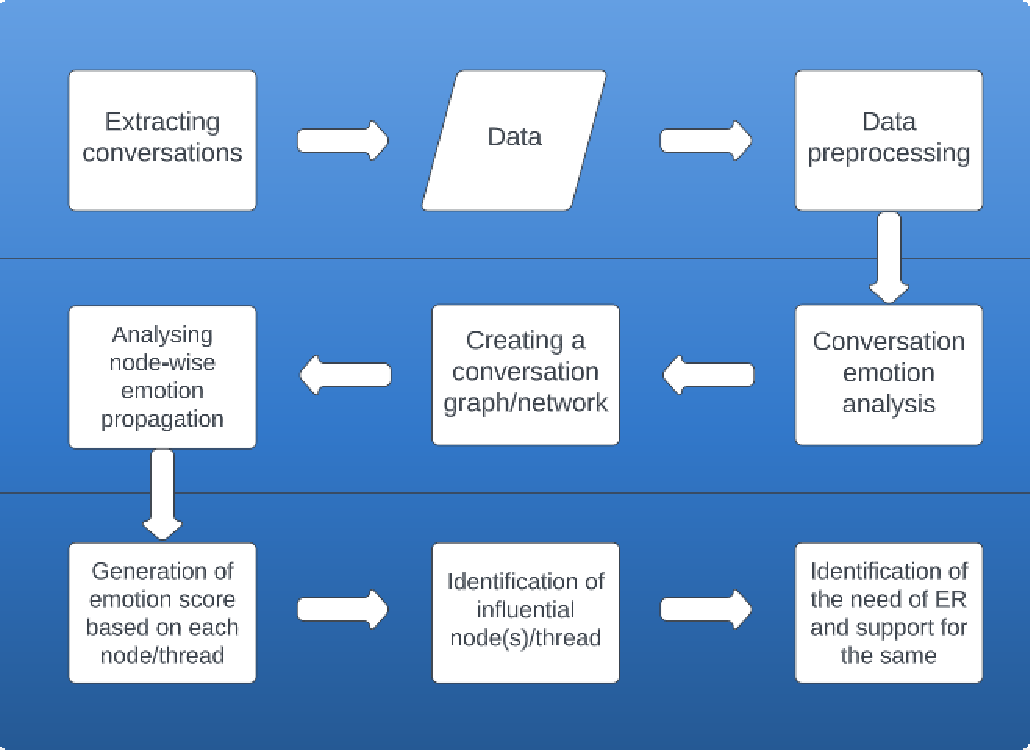
\includegraphics[width=8cm,height=8cm,keepaspectratio]{framework.pdf}
%   \includegraphics[width=5cm,height=5cm,keepaspectratio]{samples/sample_convv.png}
%   \includegraphics[width=5cm,height=5cm,keepaspectratio]{samples/sample_conv_graphh.png}
  \caption{Framework for encouraging on-spot emotion regulation in social media conversations}
  \label{fig:Framework}
  \end{figure}  
%%%%%%%%%%%%%%%%%%%


\subsection{Data}
\begin{table}[]
\centering
\caption{Parameters used to fetch tweets}
\label{tab:params}
\begin{tabular}{|p{3cm}|p{4.8cm}|}
\hline
Parameter                                         & Description                                                                                                                          \\ \hline
\texttt{author\_id}              & The unique identifier of the user who posted the tweet/comment/response.                                                             \\
\texttt{conversation\_id}        & The unique identifier used to identify a conversation/thread on Twitter.                                                             \\
\texttt{created\_at}             & Timestamp of the tweet/comment/response in UTC.                                                                                      \\
\texttt{id}                      & The unique identifier of the tweet/comment/response on Twitter                                                                       \\
\texttt{in\_reply\_to\_user\_id} & The author id of the user who received the response.                                                                                 \\
\texttt{entities}                & Provides metadata and additional contextual information about Twitter posts. For instance, hashtags, user mentions, links, and so on. \\
\texttt{lang}                    & Filter used to select English tweets.                                                                                                \\
\texttt{text}                    & The text contained in the tweet along with the emoticons.                                                                            \\ \hline
\end{tabular}
\end{table}

Twitter is regularly used by government officials in Australia, to post updates and notify of recent events or inform citizens of upcoming activities. For the purpose of this study, we analysed the tweets by Daniel Andrews, the premier of Victoria, for the period between June 2021 to August 2022. The aim was to collect a variety of conversations by topic, hashtags and context. These involved tweets about the various lockdowns, COVID vaccine updates, policy updates, local developments and announcements. A total of N conversations were selected for this analysis, each of which involved a minimum of 1000 direct responses, leading to a dataset of N*3000 rows. This data was downloaded using the \href{https://developer.twitter.com/en/docs/twitter-api}{Twitter API (Tweepy)} and the \href{https://developer.twitter.com/apitools/downloader}{tweet downloader tool} provided by Twitter. Every tweet on Twitter has a conversation ID, which was used to collect and organise tweets, comments and responses. It must be noted that each of these 50 conversations was separate tweets and not responses or quotes to another tweet. Table- \ref{tab:params} describes the parameters used while fetching the data:
% \begin{itemize}
%     \item \texttt{author\_id}
%     \item \texttt{conversation\_id}
%     \item \texttt{created\_at}
%     \item \texttt{id}
%     \item \texttt{in\_reply\_to\_user\_id}
%     \item \texttt{entities}
%     \item \texttt{lang}
%     \item \texttt{text}
% \end{itemize}


For this experiment, tweets with only text and emoticons were taken into consideration. Tweets containing images, videos or external links were not considered as it is hard to evaluate the emotions expressed in media files and links. The tweets were mostly in English, and the occasional comments in a different language were removed. The data was downloaded in the form of CSV files, one per conversation and then used for further analysis. Users involved in a conversation were identified by their \texttt{author\_id} and the \texttt{in\_reply\_to\_user\_id} was used to associate comments with its responses. The entities parameter was used to trace the sequence of responses. The number of responses to each comment and the number of unique users who responded to the comment were also added as attributes to the data. 
%%%%%%%%%%%%%%%%



\subsection{Emotion Classification}
Each row in the CSV file contained a text field representing either a tweet, a comment on a tweet or a response to a comment. The emotion expressed by the text in this field was determined using a text emotion classifier. A multi-label NLP classifier was used to categorise the tweets based on the six basic emotions (love, joy, sadness, anger, fear, and surprise). The emojis in the tweets were replaced with vector representations generated by \href{https://radimrehurek.com/gensim/}{Gensim} using the Emojinal library \cite{barry2021emojional}, after which the tweet text was tokenized using the \href{https://www.nltk.org/api/nltk.tokenize.casual.html}{TweetTokenizer}. The NLP classifier was trained and tested on the 'emotions' dataset, a two-column labelled dataset of Twitter messages with a text string and a label, it contains 20,000 rows of data \cite{saravia-etal-2018-carer}. Six emotions are described by the labels: love, joy, sadness, anger, fear, and surprise. For training, a four-layer sequential model with Bidirectional LSTM layers was used, and the data was divided 80:10:10 for training, validation, and testing. The model was trained for 20 epochs (increasing the epochs had no effect on accuracy) and achieved a testing accuracy of 87\%. The trained classifier was then used to predict the emotions expressed in the Twitter conversation. Every tweet, comment, and response in the conversation thread received an emotion label and a score, with the score indicating the probability with which the classifier predicted the emotion.
%%%%%%%%%%%%%%%%


\subsection{Graph Based Emotion Propagation Analysis}
In this work, we propose that a post or tweet is representative of the emotion it expresses as well as of the emotions expressed in its comments and responses. Hence, we calculate the overall emotion represented by a conversation, by summing up the emotional impact of its source tweet, comments and responses. A graph was generated to represent the analysis of the conversations. Networks from Online Social Networks (OSN) are commonly defined by a graph in which the nodes represent the users in the network and the edges represent the links between the nodes \cite{antonakaki2021survey}. These graphs are useful for identifying user properties such as influence, as well as network properties such as homophily. However, the goal of this study is to analyse a conversation (in which users may have participated once or multiple times) and the "impact of the users' actions" on encouraging engagement in a conversation. Rather than identifying "problematic users," the idea is to identify "posts" that are troublesome within a conversation (or that trigger anger/hate within a conversation). The general influence or behaviour profile of users on the social network was not examined for this study. We believe that informing a user of the impact of their rude comment(s) on a particular instance, rather than ticketing them as inappropriate in general, would encourage them to self-reflect on a specific case. 


It has been discovered that while public figures, media companies, and people with social influence bring a lot of initial attention to a social media post, it is the uninfluential and anonymous users who keep the engagement going and thus have a larger impact on the emotion that is propagated within a conversation \cite{solovev2022moral}, \cite{mirbabaie2021development}, \cite{saveski2021structure}. Informing users of their impact on the conversation will also question their sense of anonymity on a post and serve as a motivator to respond responsibly. As a result, for this experiment, the tweets, comments, and responses were treated as nodes in the graph, and the directed edges represented the nodes that received the responses. That is, if a comment has received n direct responses, it will have an in-degree of n. Self-loops were also present in the graph. 

\textit{\textbf{G = (V, E, A)}, where V is the set of nodes, E is the set of edges representing the nodes' existing relations, and A denotes the set of attribute vectors. The value of n=|V| represents the total number of vertices, m=|E| represents the total number of edges, and A (A1, A2, A3... Ak) associates with nodes in V and describes their characteristics.}


Finding influential nodes in a graph has been widely used in sentiment classification and the analysis of Online Social Networks (OSN). In the case of Twitter network analysis, although there is no widely accepted standard for identifying influential nodes, a combination of various connectivity/centrality-based attributes and machine learning methods has been applied \cite{berahmand2020new}, \cite{vilarinho2018global}, \cite{ban2021lexical}, \cite{bordoloi2020graph}. Because global connectivity is not a significant measure of a node's impact, in this case, attributes that focus on identifying nodes with high local impact were used. This is because two separate comments on a tweet can grow into large threads regardless of their connectivity or the presence of common nodes between them. The attributes that were used to represent the nodes are described in Table-\ref{tab:params_rule}.

\begin{table}[]
\centering
\caption{Parameters used to find influential nodes in the conversation graph}
\label{tab:params_rule}
\begin{tabular}{|p{4cm}|p{4.2cm}|}
\hline
Parameter                                         & Description                                                                                                                          \\ \hline
\texttt{number\_of\_direct\_responses}              & The in-degree of a node.                                                             \\
\texttt{total\_engagement\_received}        & The number of ancestors of a node, the number of nodes in the reply tree of a node.                                                             \\
\texttt{distance\_from\_root}             & The number of directed edges in the shortest path from a node to the root node.                                                                   \\
\texttt{page\_rank}                      & The rank of a node in the graph, based on the structure of incoming edges.                                                                      \\
\texttt{emotion\_score}                 & The probability with which the emotion classification model predicted the emotion for the text in the node.                              
                                                                         \\ \hline
\end{tabular}
\end{table}

The number of direct responses indicates a node's in-degree, and the total responses thread indicates a node's ancestors (number of nodes that have a path to the source). Pagerank is used to rank nodes with the same in-degree; (it has been preferred over betweenness centrality in this case because it estimates the nodes' local importance \cite{antonakaki2021survey}). The distance from the root is used as a factor to reinstate the distance of a trigger, a comment that initiated the reply tree is more influential than a response in the reply tree. Based on these attributes, the emotional influence of child nodes and the terminating nodes for the root node was calculated using the following rule: 
    

\textit{The impact of nodes in G = (V, E, A) on the root node R is given by:}

% 
$\forall \,V \in G-\{R\},
E(R) = \sum{E(V1, V2, V3....Vn)}
where \,E(Vi) =\prod{Ai}$

The rule is used to calculate the impact of nodes on a specific node, which in this case is the root. A threshold value was chosen based on the impact of nodes, which in this case was the mean value of node impacts on the root node. This was used to identify influential nodes, which were distinguished as nodes with a value greater than the threshold. After identifying the influential nodes \textit{(I = \{V1, V2...Vn\})} for the root node \textit{(R)}, the same rule can be used to find the nodes with the greatest impact on these influential nodes  \textit{(I = \{V11, V12...V1n\})} by considering the subgraph where the influential nodes \textit{(V1, V2..Vn)} are the root nodes.
% \end{displaymath}

% \textit{where E(Vi) = \texttt{number\_of\_direct\_responses}*\texttt{total\_engagement\_received}
% *(1/\texttt{distance\_from\_root})*\texttt{page\_rank}*\texttt{emotion\_score}}


%%%%%%%%%%%%%%%%
\subsection{Supporting On-Spot Emotion Regulation}
Conversations in the form of comments or replies to posts are a pertinent aspect of social media platforms. However, they also increase the likelihood of online hate and harassment. According to research, 41\% of US adults have been victims of online hate and harassment \cite{thomas2022s}. Hence, this work aims to break down the occurrence of hate speech in conversations by quantifying their impact on the overall conversation, so that the users can be informed about their micro-impact on a conversation and be encouraged to act responsibly.

After identifying the influential nodes in the conversation graph, the information can be used to inform users involved in the comment node's reply tree about the implications of their actions. This can be accompanied by highlighting the node based on the colour of the emotion it represents, as well as the percentage distributions of emotions, or by restricting further activity on the comment that is the reply tree's originating node. As shown in Figure-\ref{fig:Emotion}, the post has colour-coded comments and associated reply trees in conversations according to the emotions they represent, the distribution of those emotions, and the influential nodes that have a significant impact on that distribution. Nodes 3, 5 and 6 are particularly key in the conversation's anger, with node 6 having the biggest contribution. As a result, it is frozen.
\begin{figure}[h]
  
    \centering
    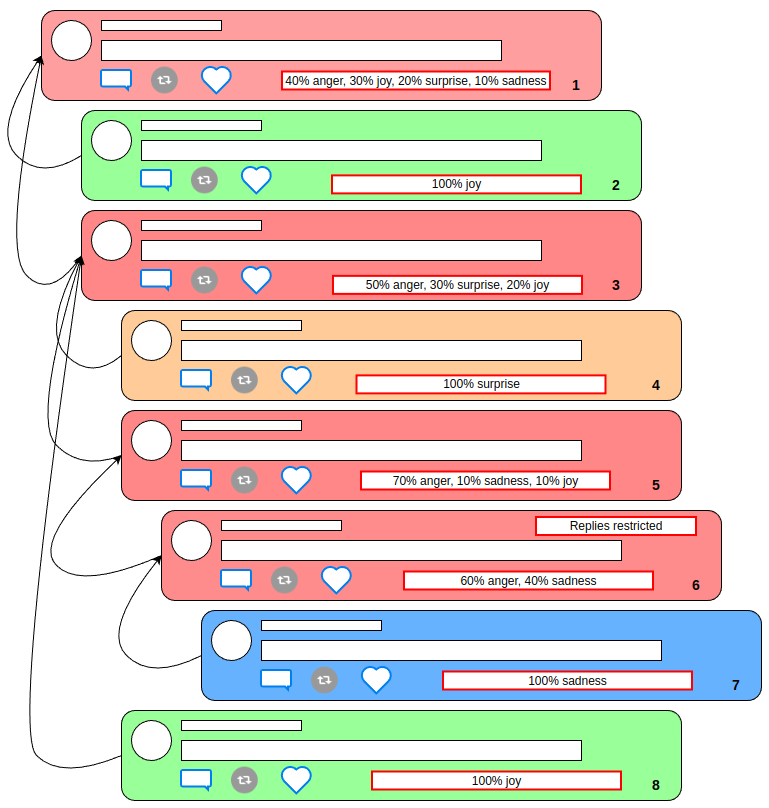
\includegraphics[width=8cm,height=8cm,keepaspectratio]{emotion_impact.png}
%   \includegraphics[width=5cm,height=5cm,keepaspectratio]{samples/sample_convv.png}
%   \includegraphics[width=5cm,height=5cm,keepaspectratio]{samples/sample_conv_graphh.png}
  \caption{Identifying influential comments/responses/threads in social media conversations. The comments are colour-coded according to the emotion they represent.}
  \label{fig:Emotion}
  \end{figure}

The decision to freeze a comment here is an attempt to identify the actions of a user or a group of users in order to avoid the post becoming hostile as a whole, as well as to decompose the toxic activity involved in a post by bringing it to light. It should be noted that suppression of anger or hate speech in this context is not the same as the inherent bias of promoting positive content on social media, but rather an attempt to avoid the induction of excessive hate on a post because it's simple to respond to a digitally induced emotional challenge with a digital action, such as expressing anger on a post by leaving an angry comment \cite{wang2021role}, \cite{smith2022digital}. The first step is self-reflection, which is similar to cognitive and dialectic behaviour therapy, which emphasises emotion regulation. Encouraging self-reflection by outlining the effects of previous user actions, will lead to a rise in awareness among the users and nudge them towards acting responsibly. 


Implicit emotion control strategies involving cognitive change, such as reappraisal or non-judgemental acceptance, can be recommended to assist the users affected by the restricted activity on their comments and prevent the creation of similar reply trees. This can be fuelled by informing users about the overall emotional distribution of the conversation in an effort to help them empathise with other participants, which will subtly prompt the user to feel responsible. This approach avoids the users from  falling into the trap of anxiety based on their general perception while their anonymity is in question since it focuses on the actions of the users rather than the users themselves. Although it is debatable if preventing additional activity on a comment creates friction for participation, it protects users' right to free speech while posing a minor distraction, and the users' freedom of choice still remains with them \cite{kiskola2021applying}. Additionally, it has been found that one of the best ways to reduce toxicity online is through the moderation of online content \cite{thomas2022s}, \cite{jhaver2021evaluating}. Questioning the users' anonymity by displaying their impact on a conversation and its emotion distribution, or freezing a particular comment in a post (depending on the length of the post, the number of persons involved, or the intensity of the emotions) serves as a modest warning of rising toxicity in this situation.



%%%%%%%%%%%%%%%%%%%%%%%%%%%%%%%%%%%%%%%%%%%%%%%%%%%%%%%%%%%%%%%%%%%%%%%%%%%%%%%%%%%%%%%%%%%%%%%%%%%%%


\begin{figure*}[h]
  \begin{minipage}{.33\textwidth}
    \centering
    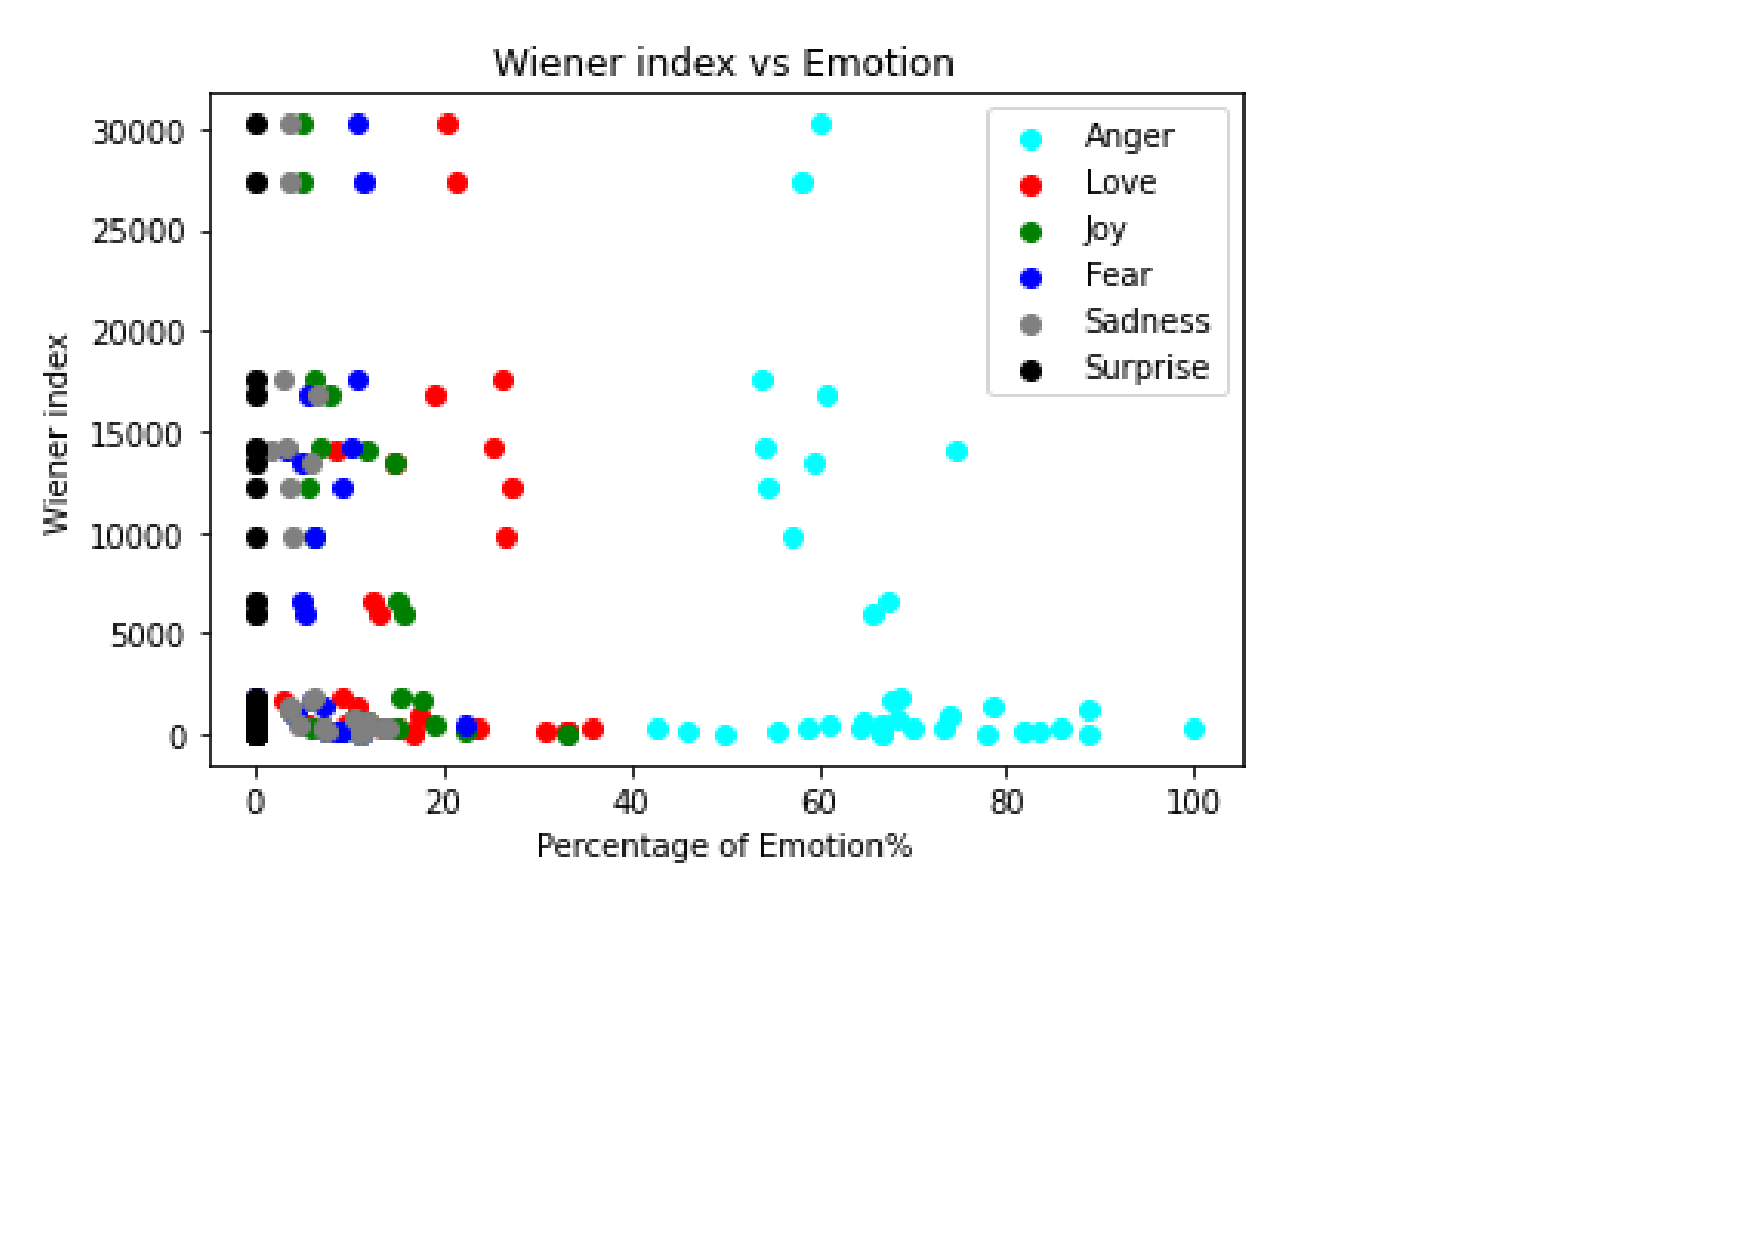
\includegraphics[width=5cm,height=5cm,keepaspectratio]{WAnger.pdf}
    \subcaption{Dominant Emotion: Anger}
  \end{minipage}%
  \begin{minipage}{.33\textwidth}
    \centering
    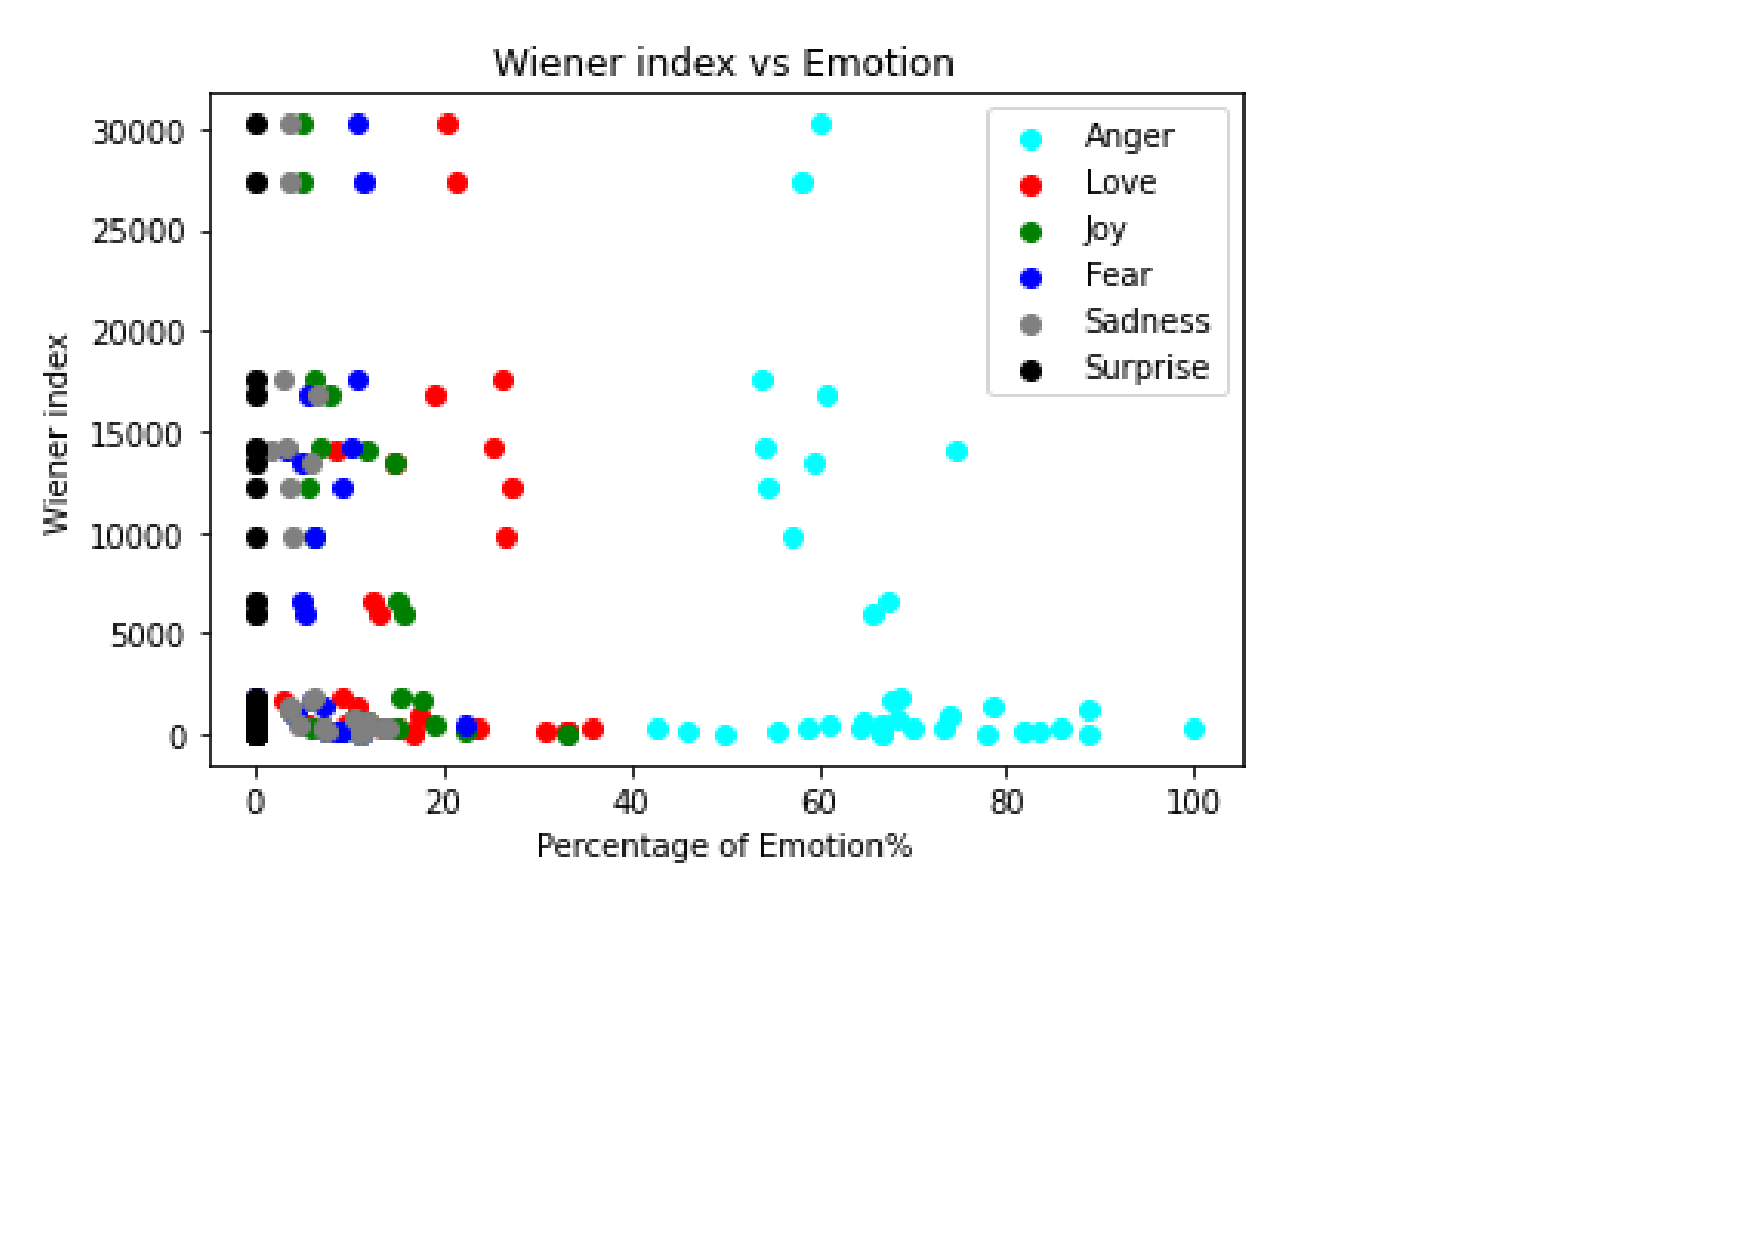
\includegraphics[width=5cm,height=5cm,keepaspectratio]{WAnger.pdf}
    \subcaption{Dominant Emotion: Anger}
  \end{minipage}%
  \begin{minipage}{.33\textwidth}
    \centering
    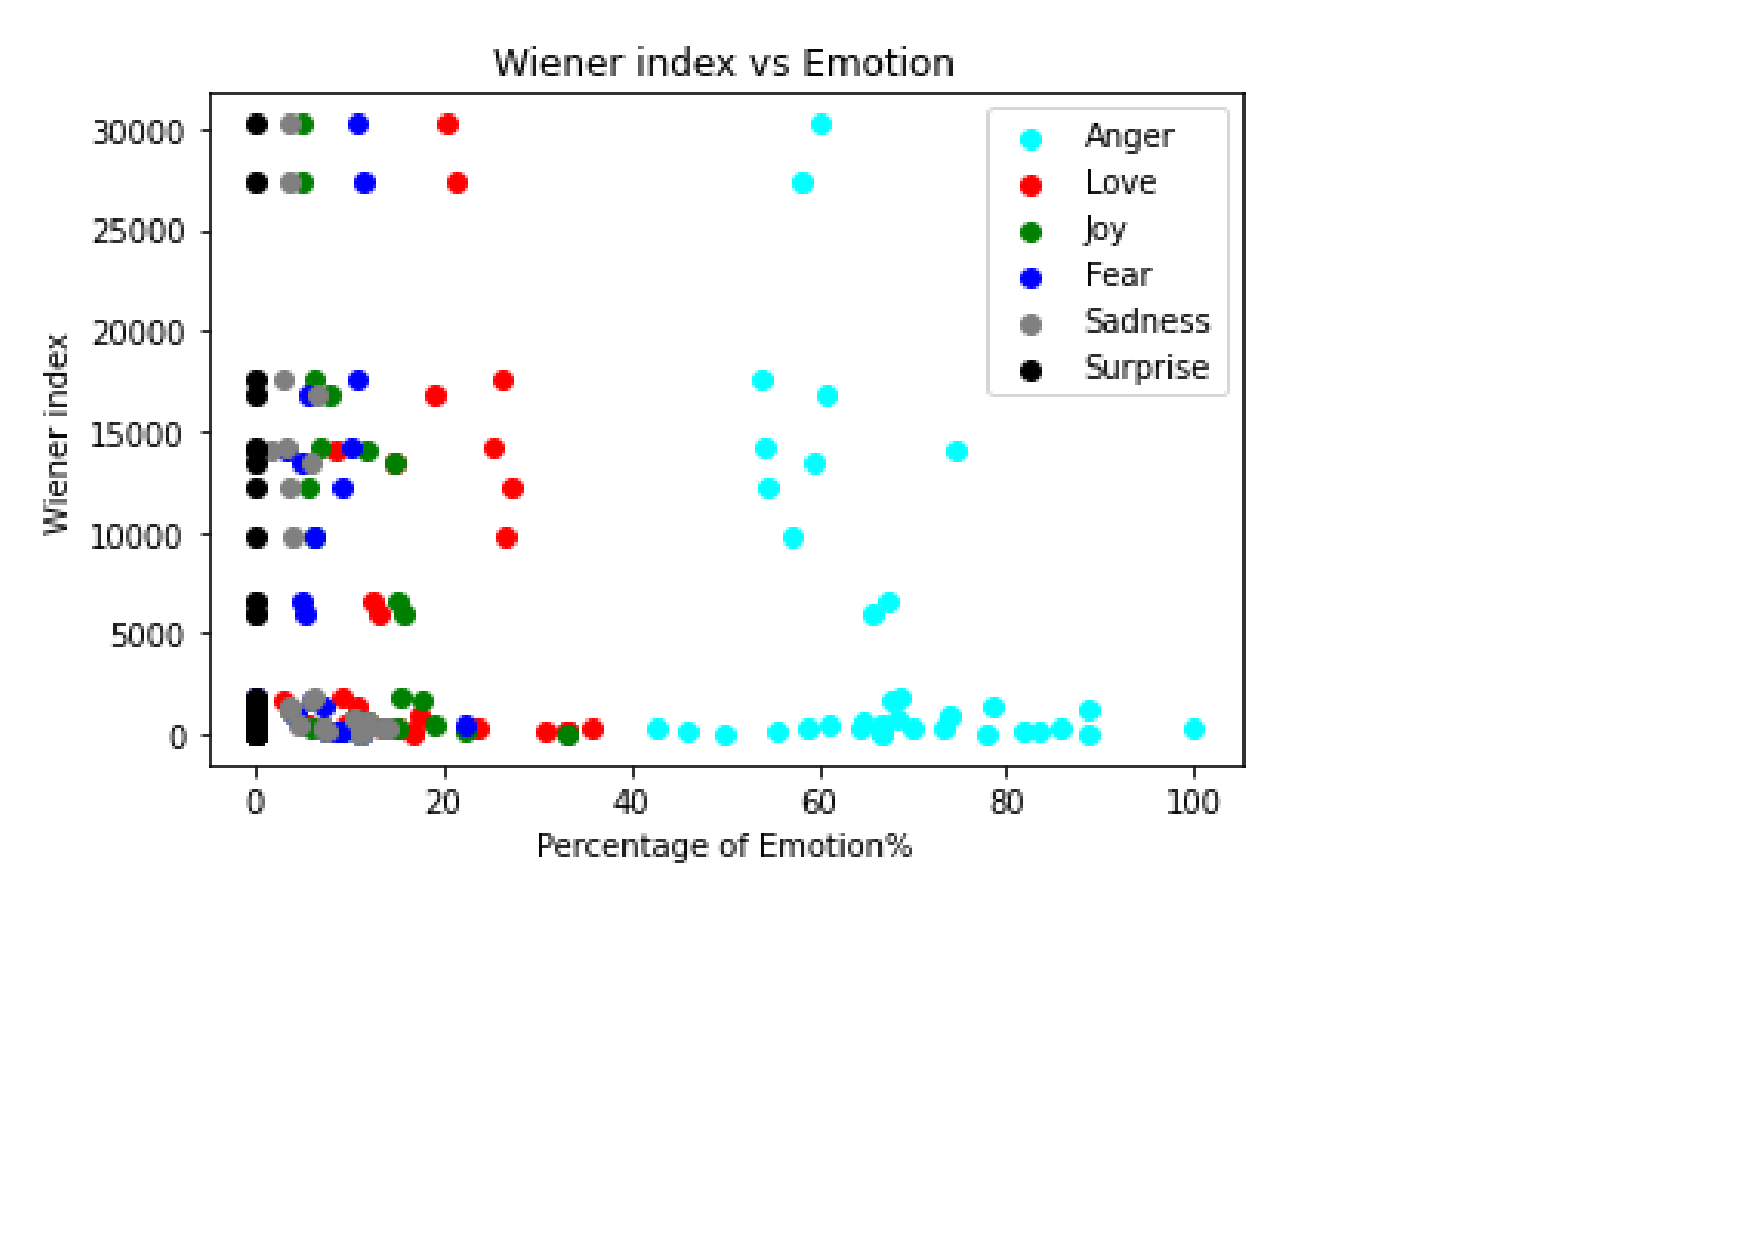
\includegraphics[width=5cm,height=5cm,keepaspectratio]{WAnger.pdf}
    \subcaption{Dominant Emotion: Anger}
  \end{minipage}
 \medskip
  \begin{minipage}{.33\textwidth}
    \centering
    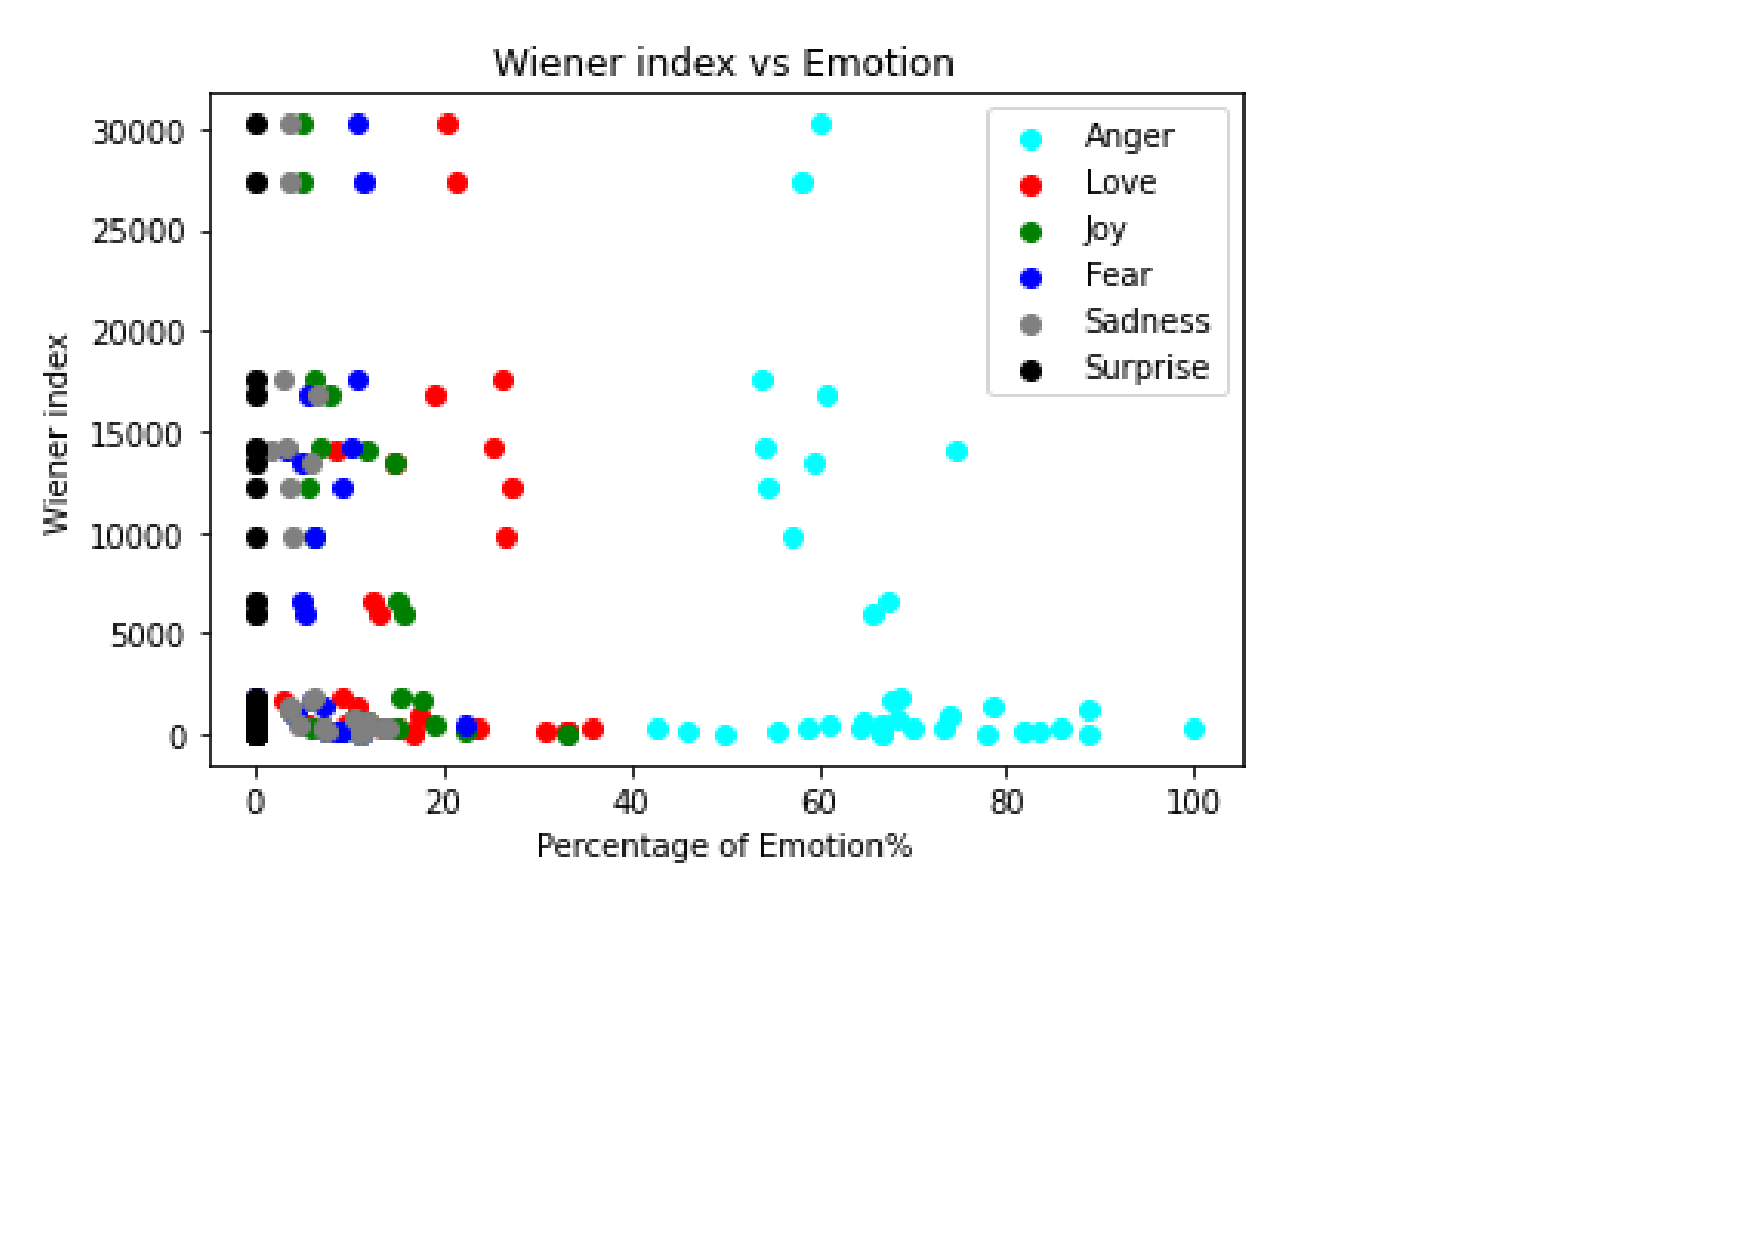
\includegraphics[width=5cm,height=5cm,keepaspectratio]{WAnger.pdf}
    \subcaption{Dominant Emotion: Anger}
  \end{minipage}%
  \begin{minipage}{.33\textwidth}
    \centering
    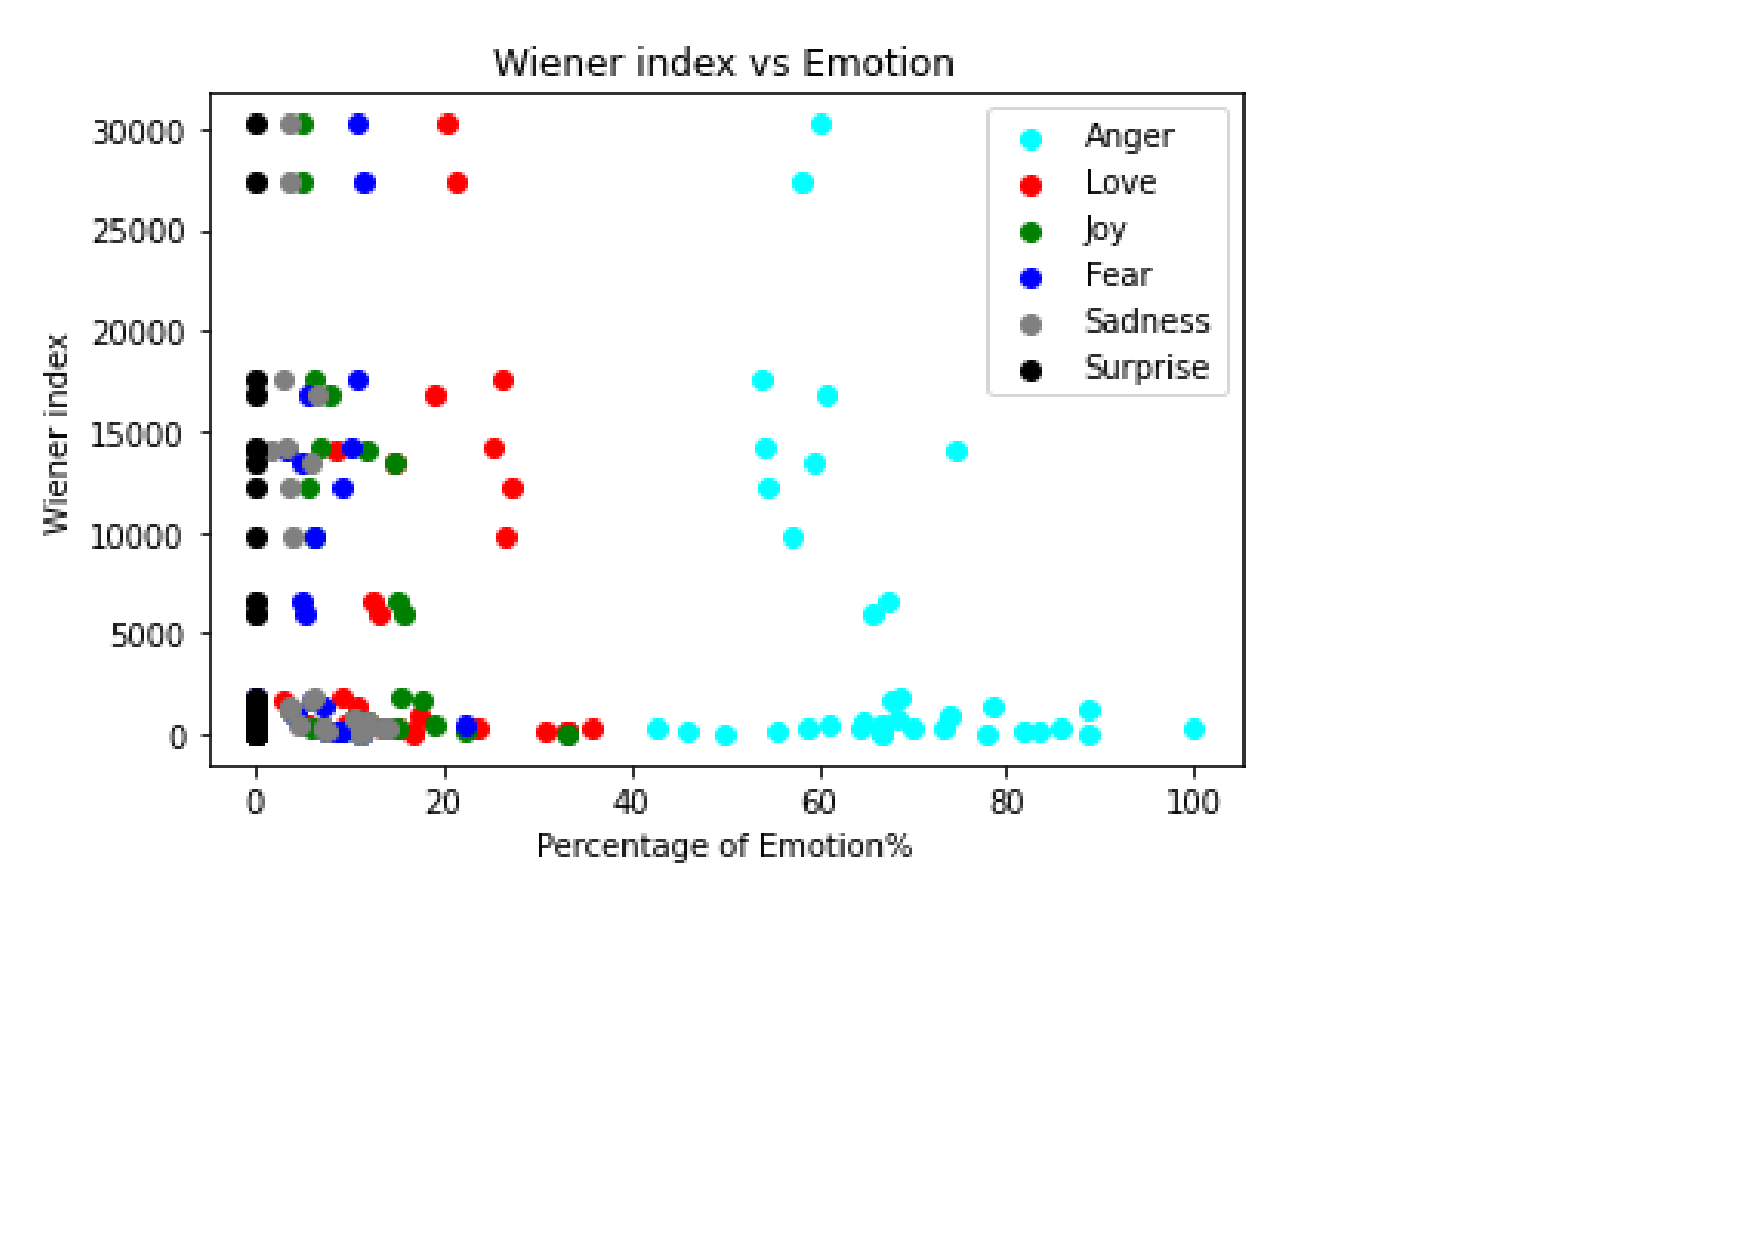
\includegraphics[width=5cm,height=5cm,keepaspectratio]{WAnger.pdf}
    \subcaption{Dominant Emotion: Anger}
  \end{minipage}
  
%   \includegraphics[width=5cm,height=5cm,keepaspectratio]{samples/sample_convv.png}
%   \includegraphics[width=5cm,height=5cm,keepaspectratio]{samples/sample_conv_graphh.png}
  \caption{Percentage distribution of emotions in the reply tree of influential nodes of conversations where the dominant emotion is (a) Anger (b) Fear (c) Sadness (d) Joy and (e) Love}
  \label{SampleConv}
  \end{figure*}
\section{Experimental Evaluation and Analysis of Emotion Propagation}
Toxicity in social media platforms has been observed in the form of hate speech, harassment, trolling and cyberbullying to name a few.  Although these harmful activities carry different intentions, they translate into action through a common pathway, that is uncivilised behaviour, more specifically uncivil language in the case of text-based social media platforms. Recent works have explored how Twitter conversations can be used to detect harassment and cyberbullying. Not only do these require contextual information and user profile data, but they are also usually applied to a conversation after it has taken place. Social media platforms have introduced moderation strategies such as deplatforming and removing inappropriate comments but they are based on static rules and are also applied after the incident has occurred. This work introduces a model to examine the propagation of emotions (through language) in online conversations in real-time. The potential of this approach lies not only in analysing if a conversation is becoming toxic but also in being able to identify why and how that is happening. Therefore, by investigating the actions that lead to toxicity, this work introduces a framework to help reduce the possibility of a conversation becoming toxic.  


In the context of Twitter, a toxic tweet can be defined as an unreasonably rude or disrespectful comment that makes a person leave the conversation. Hence, for this work, we define toxicity in a conversation as the disproportionate or excessive influx of toxic tweets/responses into an otherwise neutral post. As discussed earlier (Section 3) in this paper, we classify tweets into six emotions, (namely anger, love, joy, fear, sadness and surprise) the influx of anger has been termed as rage-inducing, rude or disrespectful and is hence seen as an indicator of toxicity.
\begin{figure*}[h]
  \begin{minipage}{.33\textwidth}
    \centering
    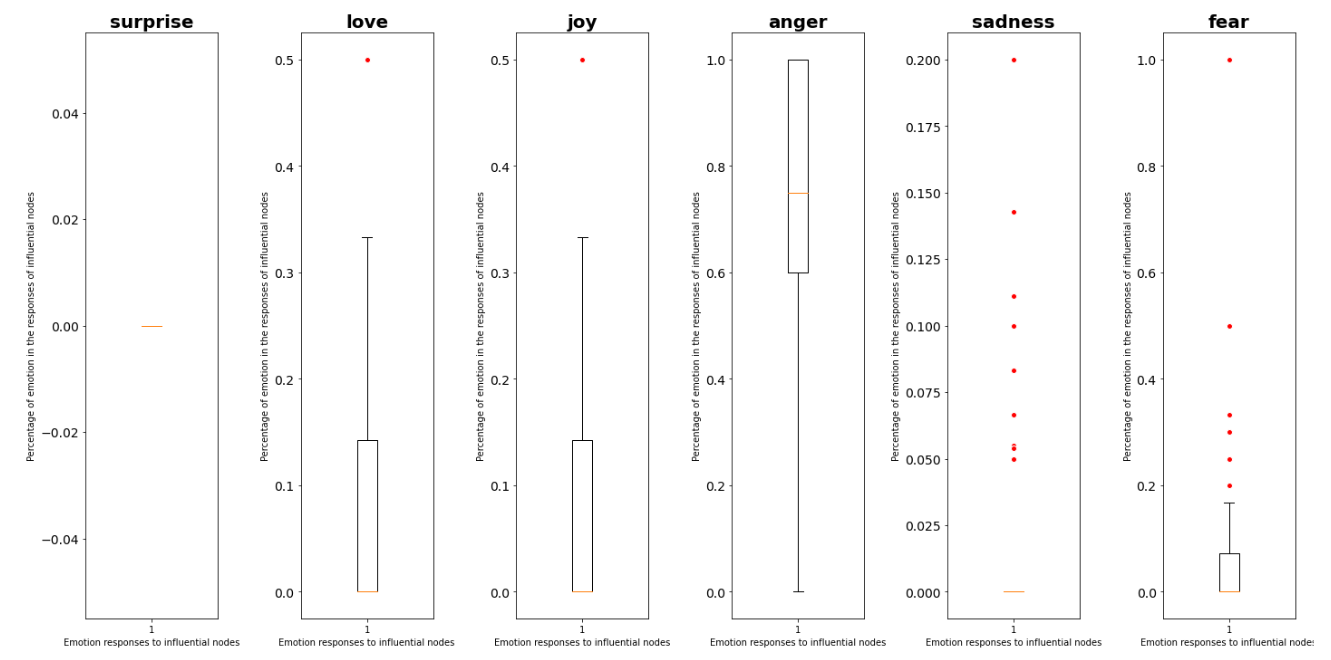
\includegraphics[width=5cm,height=5cm,keepaspectratio]{anger.png}
    \subcaption{Dominant Emotion: Anger}
  \end{minipage}%
  \begin{minipage}{.33\textwidth}
    \centering
    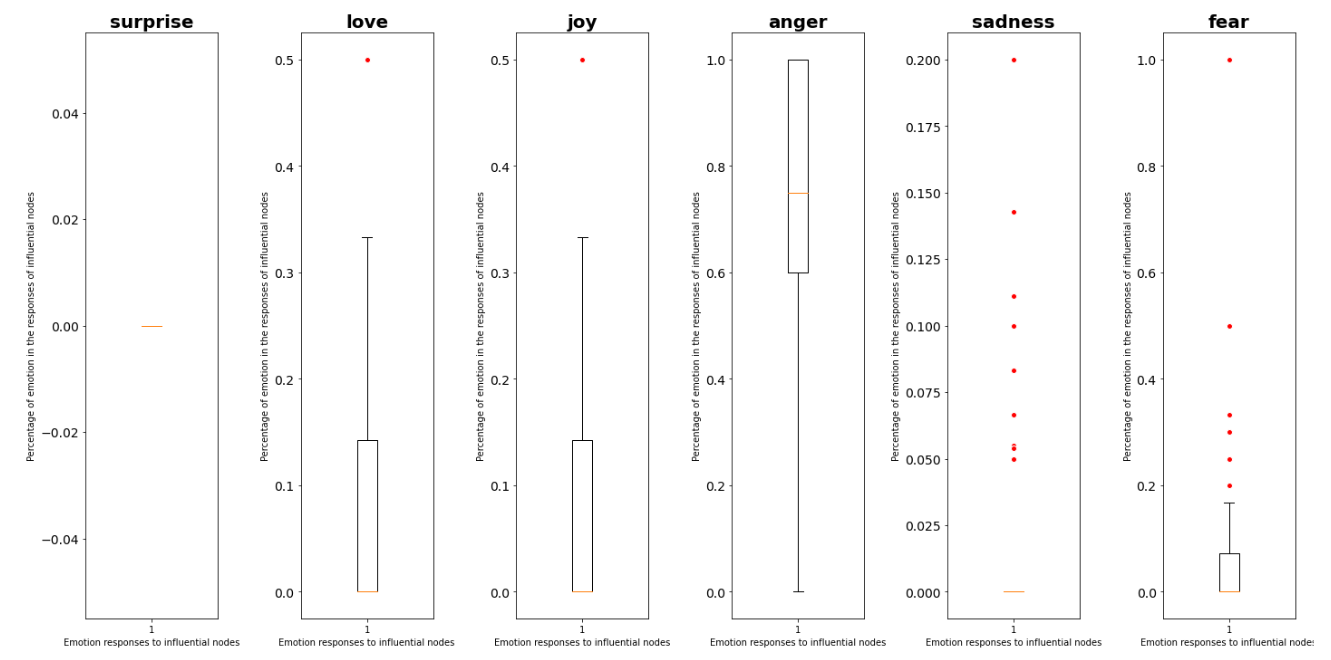
\includegraphics[width=5cm,height=5cm,keepaspectratio]{anger.png}
    \subcaption{Dominant Emotion: Anger}
  \end{minipage}%
  \begin{minipage}{.33\textwidth}
    \centering
    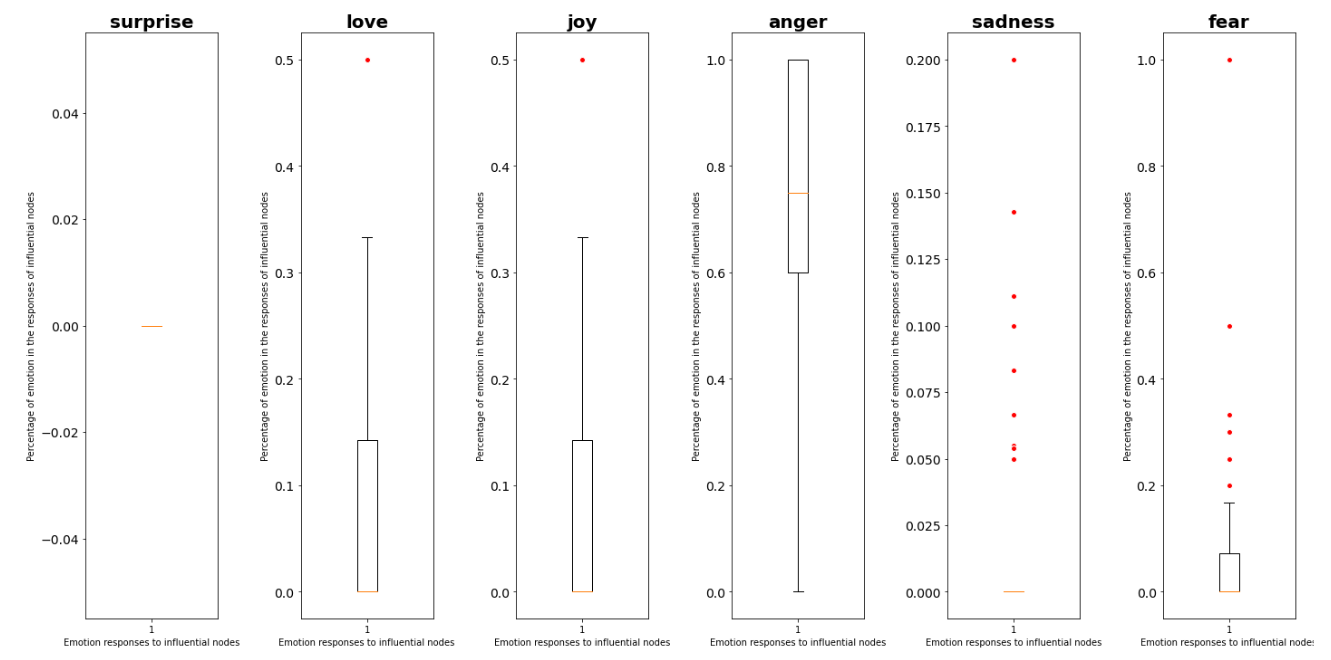
\includegraphics[width=5cm,height=5cm,keepaspectratio]{anger.png}
    \subcaption{Dominant Emotion: Anger}
  \end{minipage}
 \medskip
  \begin{minipage}{.33\textwidth}
    \centering
    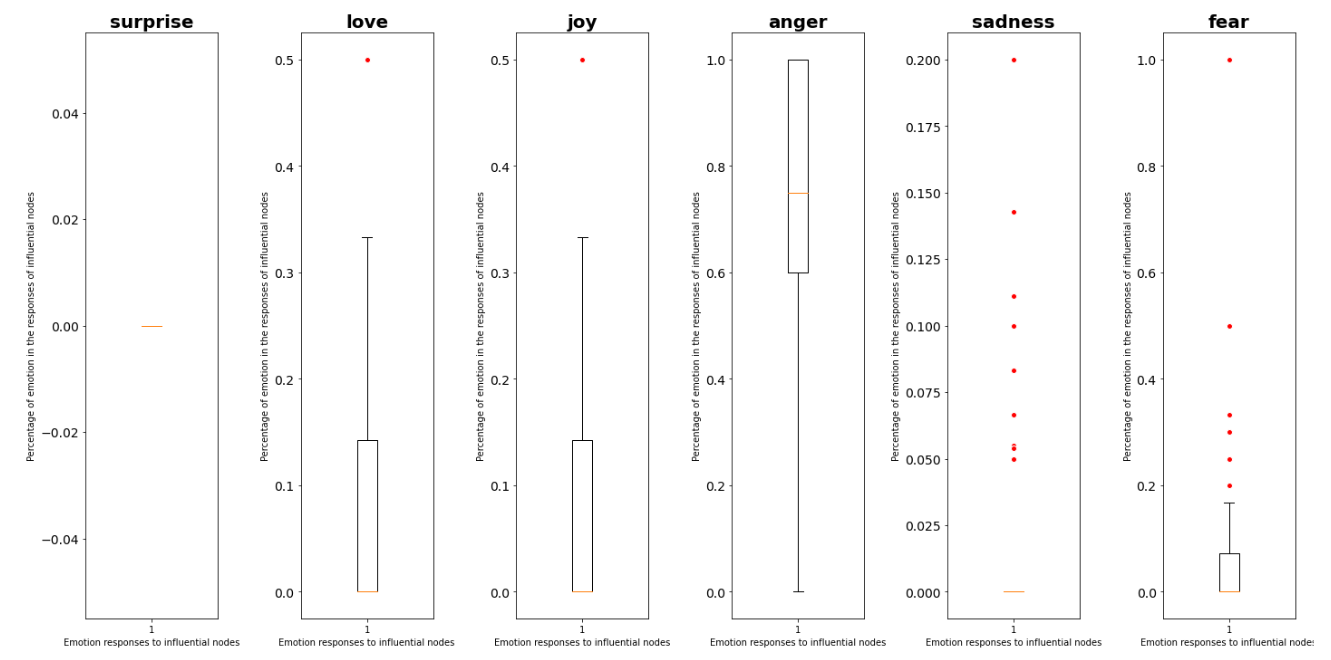
\includegraphics[width=5cm,height=5cm,keepaspectratio]{anger.png}
    \subcaption{Dominant Emotion: Anger}
  \end{minipage}%
  \begin{minipage}{.33\textwidth}
    \centering
    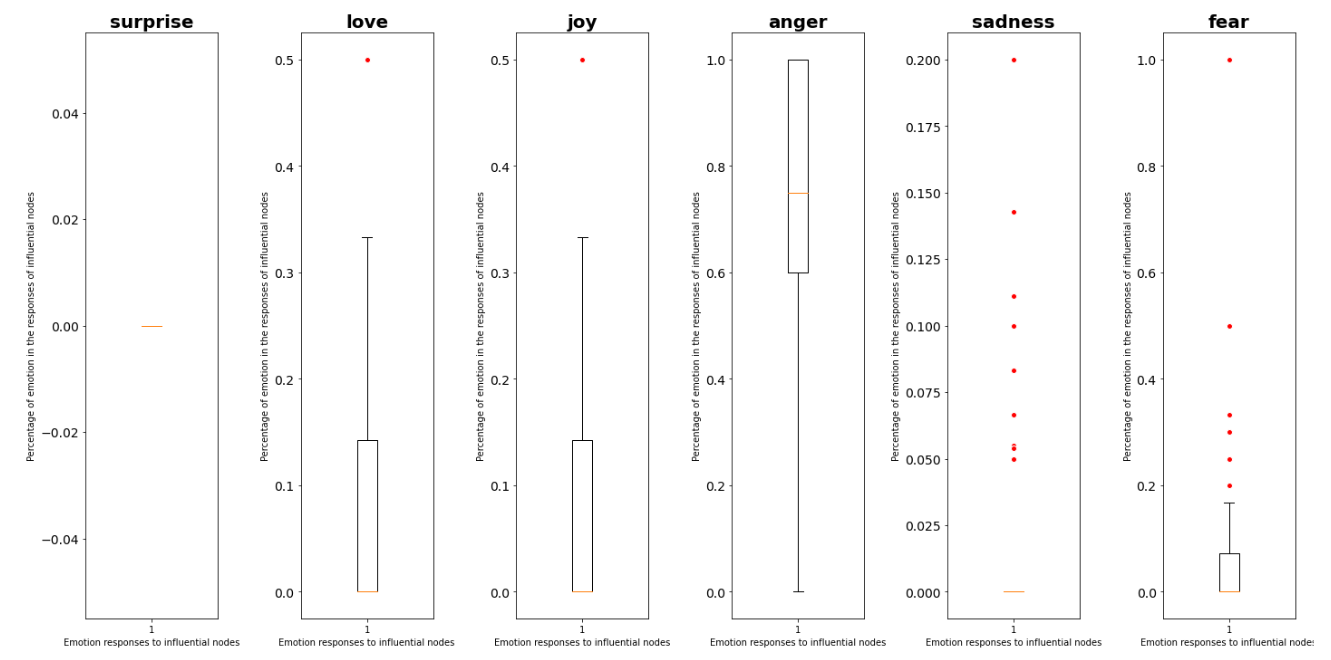
\includegraphics[width=5cm,height=5cm,keepaspectratio]{anger.png}
    \subcaption{Dominant Emotion: Anger}
  \end{minipage}
  
%   \includegraphics[width=5cm,height=5cm,keepaspectratio]{samples/sample_convv.png}
%   \includegraphics[width=5cm,height=5cm,keepaspectratio]{samples/sample_conv_graphh.png}
  \caption{Percentage distribution of emotions in the reply tree of influential nodes of conversations where the dominant emotion is (a) Anger (b) Fear (c) Sadness (d) Joy and (e) Love}
  \label{SampleConv}
  \end{figure*}
Hate speech and toxic speech have been discovered to be essential elements of virality on social media where the use of uncivil language is common to a large number of users. A viral spread corresponds to a rapid dissemination of a piece of information via connective action of users and is often fuelled by the emotions it entails. Studies have shown that both hate speech and toxicity spiral in action which leads to a faster and more widespread dispersal. Hence, by keeping an eye on the nature of information diffusion as well as the compounding effect of emotion propagation within a conversation graph, it is possible to identify when and how a conversation may become toxic and thus apply moderation strategies before it turns toxic. The same can also be used to determine the need for emotion regulation. The focus here is to inform users involved in a conversation about their emotional impact and gently nudge them towards a responsible mindset through repetitive application of the same. 
The structure and toxicity of Twitter conversations have been widely studied. We utilise findings from these studies to validate the applicability of our framework. We do so based on three attributes, structural characteristics, emotions and virality, and the development of connective action.
% Please add the following required packages to your document preamble:
% \usepackage{graphicx}
\begin{table}[]
\caption{}
\label{tab:my-table}
\resizebox{\columnwidth}{!}{%
\begin{tabular}{p{2.5cm}|p{2.5cm}|p{2.5cm}|p{2cm}}
\hline
Utilised Model &
  Identification of influential nodes &
  \begin{tabular}[c]{@{}l@{}}Percentage of nodes\\  identified as toxic\end{tabular} &
  \begin{tabular}[c]{@{}l@{}}Percentage reduction in\\ toxicity if acted on\\ these nodes\end{tabular} \\ \hline
Proposed Framework &
  \begin{tabular}[c]{@{}l@{}}On the basis of impact score,\\ taking into account the \\ comment/reply/tweet text \\ as well as its connectivity\end{tabular} &
  1-4\% &
  10\% \\ \hline
Perspective API & \begin{tabular}[c]{@{}l@{}}On the basis of toxicity, taking\\ into account only the \\ comment/reply/tweet text\end{tabular}      & 1-2\% & 7\%  \\ \hline
Combination     & \begin{tabular}[c]{@{}l@{}}Takes into account the emotion\\  in the text, the connectivity\\ as well as its toxicity\end{tabular} & 1-4\% & 12\% \\ \hline
\end{tabular}%
}
\end{table}
Structural characteristics: When a user posts a tweet, other users may respond to the tweet by liking, sharing or commenting on the tweet which can lead to subsequent replies. The resultant is a conversation graph with the reply trees rooted in the original tweet. Toxicity has been shown to rise with the increase in the size, density and width of a conversation graph. As can be seen from Table 4, as the size of the conversation increases, it tends to be dominated by a single emotion that has been expressed the most as opposed to the initial distribution of emotions. If we consider the toxicity of a reply tree to be the fraction of toxic tweets it receives, it can be seen rising with the size, width as well as density of the reply tree. The percentage of angry responses on the tweet skyrockets at 40\% and goes on increasing until it plateaus at 80\%. Since anger is also found to spread faster than other emotions, the same can also be observed here when comparing the ratio of the percentage of emotions contained in the nodes to the total number of nodes in the graph. Recently Wiener index has been applied to study the structure of information diffusion, particularly for characterising whether information spreads in a broadcast or viral manner. The Wiener index w(T) of a reply tree T is defined as the average distance between all pairs of nodes. A low Wiener index is associated with the broadcast structure of diffusion in which users mostly respond to the original tweet and there is minimal engagement within the users whereas a high value of the Wiener index relates to a viral spread wherein the instances of back-and-forth engagement among the users are higher than the responses to the original tweet. After finding the influential nodes of the conversation graph, we calculated the Wiener index of these nodes with respect to the percentage of emotions contained in their reply trees. It was observed that the Wiener index for anger cultivates the highest. It is initially low and starts to rise as the percentage of anger in the reply tree grows. It peaks when the nodes in the reply tree constitute 60\% anger and then drop by a small value, ultimately plateauing in the end. This brings us to the conclusion that initially, the influential node was broadcasting a variety of emotions, and as the size of its reply tree and the percentage of anger grows, it turns into a viral spread where the back-and-forth engagement received by the nodes of this reply tree increases. Thereafter, once the percentage of anger becomes 60\%, due to the back-and-forth engagement in multiple nodes of this reply tree, the nodes start broadcasting the same emotion and hence pivot into a toxic conversation as the conversation is now concentrated in these few nodes leading to the propagation of anger. Although the pattern of the conversation pivoting from broadcast to viral and back to broadcasting can be observed across other emotions as well, it was also seen that the peaks converge a lot sooner (35-40\%) and at a value higher (second-order of magnitude) than anger. It reiterates the fact that anger spreads faster by converging to virality and broadcasting sooner. These results are in line with the findings in the literature and hence validate the applicability of our hypothesis.

Emotions and virality: The success of online content nowadays relies upon how well it can influence others. This is also the motivation behind online posts and a factor to increase one's reach. When analysing the user activity in the influential nodes, it was observed that the number of responses a tweet receives is directly proportional to the amount of emotion contained in the tweet. Although tweets that expressed anger and love received the maximum responses, most of these responses were angry. Moreover, the number of angry or rage-induced responses received by a tweet that expressed love was the highest. On further analysis, it was found that these responses came from repetitive replies by the same group of users. It was observed that these responses created a polarising effect, that seemed to amplify by the repetitive participation of users who identify with the idealogy, thus creating hostility against any other emotion. A similar polarisation has been observed in literature where other-condemning emotions embedded in tweets, start the rumour cascade and may function as accelerators for the spread. This would imply that radical ideas and beliefs are strengthened and are more likely to translate into toxicity. Given increased ideological polarization, the explosive mix of other-condemning emotions should thus accelerate their spread within social networks. From Table 3, it can also be seen that the average increase in the percentage of nodes exhibiting anger after the calculation of the emotion propagation is higher as compared to other emotions. The difference also lies in the ratio of the number of angry responses received by an angry comment versus a comment expressing any other emotion. This was true not only for all cases in our study but across the six emotions. Figure 3 demonstrates the percentage increase in the emotion exhibited by the nodes in the conversation graph after the propagation has been calculated.
Development of Connective Action: Social media is now a platform for social movements that evolve under the scope of connective action. It is through user engagement that the activity of a post takes action and is maintained. anonymous users keep the activity high. It has been discovered that toxicity on a post comes from the uninfluential and the unrelated. Journalists, celebrities and other public personalities may catalyse the initial popularity of a tweet but have been found to mostly post promotional content. It is the private persons or general users that not only maintain the engagement of a post but also induce hate speech or toxicity. This could be because the main objective of Private Persons is to utilize the platform to express and connect themselves. Since they are not the most retweeted or popular, emotional expression becomes their medium of getting their ideas into the public eye. Therefore, their anonymous actions are the driving force for a post. This also fits well with Castells’ [15] idea of emotional mobilization, which is said, among the psychological states of a collection of individuals, to be essential for starting a social movement. The wording of Milano’s tweet contained both the necessary outrage and the hope for possible change.
This calls for handling the imbalanced induction of anger on social media posts in a sensitive manner that is not just suppression. Deplatforming or banning a user from making further comments may reduce the amount of anger on a post temporarily but does little in the long term since it does not serve to solve the root cause of irresponsible behaviour. Since widespread toxicity is caused by collection action, analysing the propagation of emotions based only on user actions rather than users, in general, will help lessen actions that lead to toxicity. Therefore, diluting the anonymity of users by exposing the impact of their actions will encourage implicit emotion regulation,  provoking self-reflection and responsible behaviour. 




Apart from the prevention of compounding anger or hate speech in general that later becomes toxic, this framework takes into account the subjectivity of toxicity by not relying on only the content of a post/reply/comment and taking into account its impact on the ongoing conversation. We evaluated our framework by comparing it with the toxicity scores generated by the Google Perspective API. The Perspective API provides information about the potential impact of a comment on a conversation by providing a score for the "toxicity" of a comment. We used the AnalyseComment attribute to extract the toxicity in a comment, which returns a probability score (a value in the range of 0-1). The score reflects the percentage of readers who would perceive the comment as toxic. For the sake of uniformity across our experiments, we calculated a threshold value for toxicity (0.9), based on the mean value reported in the analysis. This value of the threshold is also recommended by the Perspective API for the purpose of research, a high value minimises the potential for bias. Thereafter, we classified a tweet/comment as toxic according to this threshold value. When analysing the conversation for the presence of toxicity, it was observed that not only the most toxic tweets/comments were also some of the influential nodes, but more than 87\% of toxicity of an overall conversation was concentrated in the reply tree of influential nodes. Since the aim is to reduce the induction of hate speech in a conversation, by analysing its influential nodes, we used to toxicity score from the Perspective API to find the influential nodes. Thereafter, we used a combination of our rule and the toxicity scores to find influential nodes within a conversation. We observed that while there is a 75\% match in the influential nodes generated by our framework and the Perspective API, there exists a 94.3\% match in the influential nodes generated by the combination of the framework and the API. This confirms that the proposed framework can be used to identify comments which may be adding to the toxicity of a post while considering their subjectivity and regardless of whether or not they're individually toxic. This framework can be utilised in conjunction with APIs like AnalyseComment so that the content and context are both taken into account for the purpose of understanding the source(s) of toxicity in conversations.

We also analysed the amount of hate speech that can be curbed by de-activating the influential nodes or restricting further activity on these nodes after they reach the threshold of toxicity. We found that while our model could be used to reduce the occurrence of hate speech by 10\%, and the Perspective API by 7\%, the combination of our model and the API can be used to reduce the toxicity by 15\%. This goes hand in hand with the understanding that restricting activity on a comment may not stop users from commenting elsewhere or creating a new thread on the same post, but since the restriction is accompanied by factual information of one's impact on the post, we believe it will encourage self-reflection and implicit emotion regulation by repeated application.





\subsection{Performance Metrics}
%%%%%%%%%%%%%%%%%%%%%%%%%%%%%%%%%%%%%%%%%%%%%%%%%%%%%%%%%%%%%%%%%%%%%%%%%%%%%%%%%%%%%%%%%%%%%%%%%%%%%






\section{Conclusion and Future Work}

%%%%%%%%%%%%%%%%%%%%%%%%%%%%%%%%%%%%%%%%%%%%%%%%%%%%%%%%%%%%%%%%%%%%%%%%%%%%%%%%%%%%%%%%%%%%%%%%%%%%%



\section{Rights Information}







\section{Citations and Bibliographies}



\section{Acknowledgments}







%%
%% The acknowledgments section is defined using the "acks" environment
%% (and NOT an unnumbered section). This ensures the proper
%% identification of the section in the article metadata, and the
%% consistent spelling of the heading.


%%
%% The next two lines define the bibliography style to be used, and
%% the bibliography file.
\bibliographystyle{ACM-Reference-Format}
\bibliography{refs}

%%
%% If your work has an appendix, this is the place to put it.
\appendix


\end{document}
\endinput
%%
%% End of file `sample-acmtog.tex'.
